\documentclass[conference]{IEEEtran}
\IEEEoverridecommandlockouts
% The preceding line is only needed to identify funding in the first footnote. If that is unneeded, please comment it out.
\usepackage{cite}
\usepackage{amsmath,amssymb,amsfonts}
\usepackage{algorithmic}
\usepackage{graphicx}
\usepackage{textcomp}
\usepackage{xcolor}
\def\BibTeX{{\rm B\kern-.05em{\sc i\kern-.025em b}\kern-.08em
    T\kern-.1667em\lower.7ex\hbox{E}\kern-.125emX}}

\makeatletter
\renewcommand{\maketag@@@}[1]{\hbox{\m@th\normalsize\normalfont#1}}%
\makeatother
\begin{document}

%\title{Conference Paper Title*\\
%{\footnotesize \textsuperscript{*}Note: Sub-titles are not captured in Xplore and
%should not be used}
%\thanks{Identify applicable funding agency here. If none, delete this.}
%}
%
%\author{\IEEEauthorblockN{1\textsuperscript{st} Given Name Surname}
%\IEEEauthorblockA{\textit{dept. name of organization (of Aff.)} \\
%\textit{name of organization (of Aff.)}\\
%City, Country \\
%email address or ORCID}
%\and
%\IEEEauthorblockN{2\textsuperscript{nd} Given Name Surname}
%\IEEEauthorblockA{\textit{dept. name of organization (of Aff.)} \\
%\textit{name of organization (of Aff.)}\\
%City, Country \\
%email address or ORCID}
%\and
%\IEEEauthorblockN{3\textsuperscript{rd} Given Name Surname}
%\IEEEauthorblockA{\textit{dept. name of organization (of Aff.)} \\
%\textit{name of organization (of Aff.)}\\
%City, Country \\
%email address or ORCID}
%\and
%\IEEEauthorblockN{4\textsuperscript{th} Given Name Surname}
%\IEEEauthorblockA{\textit{dept. name of organization (of Aff.)} \\
%\textit{name of organization (of Aff.)}\\
%City, Country \\
%email address or ORCID}
%\and
%\IEEEauthorblockN{5\textsuperscript{th} Given Name Surname}
%\IEEEauthorblockA{\textit{dept. name of organization (of Aff.)} \\
%\textit{name of organization (of Aff.)}\\
%City, Country \\
%email address or ORCID}
%\and
%\IEEEauthorblockN{6\textsuperscript{th} Given Name Surname}
%\IEEEauthorblockA{\textit{dept. name of organization (of Aff.)} \\
%\textit{name of organization (of Aff.)}\\
%City, Country \\
%email address or ORCID}
%}
\title{RFC-HyPGCN: A Runtime Sparse Feature Compress Accelerator for Skeleton-Based GCNs Action Recognition Model with Hybrid Pruning
\thanks{Identify applicable funding agency here. If none, delete this.}
}
%
%\author{\IEEEauthorblockN{1\textsuperscript{st} Given Name Surname}
%\IEEEauthorblockA{\textit{dept. name of organization (of Aff.)} \\
%\textit{name of organization (of Aff.)}\\
%City, Country \\
%email address or ORCID}
%\and
%\IEEEauthorblockN{2\textsuperscript{nd} Given Name Surname}
%\IEEEauthorblockA{\textit{dept. name of organization (of Aff.)} \\
%\textit{name of organization (of Aff.)}\\
%City, Country \\
%email address or ORCID}
%\and
%\IEEEauthorblockN{3\textsuperscript{rd} Given Name Surname}
%\IEEEauthorblockA{\textit{dept. name of organization (of Aff.)} \\
%\textit{name of organization (of Aff.)}\\
%City, Country \\
%email address or ORCID}
%\and
%\IEEEauthorblockN{4\textsuperscript{th} Given Name Surname}
%\IEEEauthorblockA{\textit{dept. name of organization (of Aff.)} \\
%\textit{name of organization (of Aff.)}\\
%City, Country \\
%email address or ORCID}
%\and
%\IEEEauthorblockN{5\textsuperscript{th} Given Name Surname}
%\IEEEauthorblockA{\textit{dept. name of organization (of Aff.)} \\
%\textit{name of organization (of Aff.)}\\
%City, Country \\
%email address or ORCID}
%\and
%\IEEEauthorblockN{6\textsuperscript{th} Given Name Surname}
%\IEEEauthorblockA{\textit{dept. name of organization (of Aff.)} \\
%\textit{name of organization (of Aff.)}\\
%City, Country \\
%email address or ORCID}
%}

\maketitle

\begin{abstract}
%This document is a model and instructions for \LaTeX.
%This and the IEEEtran.cls file define the components of your paper [title, text, heads, etc.]. *CRITICAL: Do Not Use Symbols, Special Characters, Footnotes,
%or Math in Paper Title or Abstract.

Skeleton-based Graph Convolutional Networks (GCNs) models for action recognition have achieved excellent prediction accuracy in the field. However, limited by large model and computation complexity, GCNs for action recognition like 2s-AGCN have insufficient power-efficiency and throughput on GPU. Thus, the demand of model reduction and hardware acceleration for low-power GCNs action recognition application becomes continuously higher.

To address challenges above, this paper proposes a runtime sparse feature compress accelerator with hybrid pruning method: RFC-HyPGCN. The hybrid pruning approach includes dataflow reorganization and mixed-grained pruning means. By reorganizing the multiply order, this method skips both graph and spatial convolution workloads. Following spatial convolution��s channel-pruning dataflow, a coarse-grained pruning method on temporal filters is designed, together with sampling-like fine-grained pruning on time dimension. Later, we come up with an architecture with all convolutional layers mapped on chip to pursue high throughput. The scale of storage elements and computing units for each layer are specifically tuned to match the pruned model. To further reduce storage resource utilization, online sparse feature compress format is put forward. Feature is divided and encoded into several banks according to presented format, then bank storage is split into depth-variable mini-banks. In this way, the runtime compress method not only decreases useless storage, but also gets better storage regularity over compressed sparse columns format (CSC). Furthermore, this work applies quantization, input-skipping and intra-PE dynamic data scheduling to accelerate the model. In experiments, pruning method above is conducted on 2s-AGCN, acquiring 3.0x~8.4x model compression ratio and 73.20\% graph-skipping efficiency with no accuracy loss. Moreover, our pruning method ensures a hardware-friendly weight-static dataflow. Implemented on Xilinx XCKU-115 FPGA, the proposed architecture has the peak performance of 1142 GOP/s and achieves 9.59x and 2.56x speedup over high-end GPU Nvidia 2080Ti and Nvidia V100, respectively. Compared with latest accelerator for action recognition GCNs models, our design reaches 22.9x speedup and 28.93\% improvement on DSP efficiency.
\end{abstract}

\begin{IEEEkeywords}
component, formatting, style, styling, insert
\end{IEEEkeywords}

\section{Introduction}
%This document is a model and instructions for \LaTeX.
%Please observe the conference page limits.
Action recognition based on deep learning has the great potential being applied in kindergartens, hospitals and stadiums to prevent danger motions. Skeleton-based graph convolutional networks (GCNs) methods have achieved state-of-the-art (SOTA) prediction accuracy in the field \cite{}. Mature pose estimation algorithms extract human skeletons from video stream with real-time speed, for example, Open pose \cite{} and Alpha pose \cite{}. GCNs action recognition models and pose estimation models thus can combine into an end-to-end system.

Despite skeleton-based GCNs having great advantages, several problems limit their applications in expected scenarios. Firstly, intensive computation and large network architectures are embedded in skeleton-based GCNs, causing great computing cost on GPU. Mobile pose \cite{} can produce human skeletons on mobile platform Snapdragon 845 with 60 fps and 44.4 fps/Watt, while 2s-AGCN model merely has a performance of 28 fps and 0.11fps/Watt on Nvidia's 2080Ti GPU. The computing speed and power-consumption's gap indicates a great importance on accelerating GCNs action recognition algorithms. Secondly, the expected application environment of action recognition models poses stringent constraints on power-consumption and throughput. However, the high-performance GPU cannot meet the power-efficiency demand.

Network pruning and graph sparsification\cite{bianchi2020hierarchical} are two effective methods to relieve model's complexity. However, these methods are unsuitable for skeleton-based GCNs. There are two reasons. (i) \emph{Dataflow is transformed}: Graph computation is introduced to raise prediction performance but changes the dataflow at the same time. When being conducted on different dataflows, traditional pruning methods for CNNs may not achieve the same computation-skipping efficiency. (ii) \emph{Skeleton-relationship graph is unchangeable and sensitive.} Some works use pooling \cite{} or graph sparsification \cite{} to drop unimportant edges and points to decrease the scale of computation. However, the human skeleton graph cannot be modified from the view of Physiology for human bones and joints' connection being unchangeable. Particularly, in some GCNs models there exist learnable hidden information graph \cite{shi2019two}, which lacks sparsity. The subtle elements in such graph are proved to be positively associated with prediction performance, for instance in 2s-AGCN model, the prediction accuracy decreases by 2.3\% without learnable matrix \cite{shi2019two}.

Although there are many hardware accelerators for sparse CNNs and GCNs, previous works are not likely to be the best choice for high-throughput GCNs action recognition architecture. On the one hand, sparse CNNs accelerator is established on pruned models and computation reduction, but as is stated above, such pruning method cannot skip graph computation efficiently. On the other hand, previous GCNs�� accelerators focus on utilizing the sparsity in target graph and on keeping a balancing workload dispatch. Meanwhile, data sparsity in action recognition GCNs is derived from feature and pruned weight, not the graph.

For these reasons, efficient pruning methods together with specific accelerator designs are urgently required to accelerate GCNs action recognition workloads. We therefore present RFC-HyPGCN: a runtime sparse feature compress accelerator for skeleton-based GCNs action recognition model with hybrid pruning in this paper.

A hybrid GCNs�� pruning method is proposed, which can reduce convolutional parameters as well as skipping graph computation efficiently. We reorganize dataflow by changing the multiply order of graph workloads and spatial convolution. With new dataflow, a group of graph computation and spatial convolution is skipped if the corresponding parameter is pruned as zero. As to temporal convolution, multi-grained pruning method is elaborately designed. Fine-grained pruning operation can be dealt as whether to sample current data in time series, while coarse-grained pruning is decided by spatial convolution��s pruned dataflow. The experiments demonstrate that better prediction accuracy and hardware-friendly feature can be possessed by our pruned model compared with conventional pruning methods under the same compress ratio. Additionally, quantization and input-skipping are applied on software level.

We also design an application-specific architecture, where ten convolution blocks are mapped on FPGA, which is widely used for accelerating deep neural networks. Different from previous works, in our layer-pipelined architecture, challenges are not only reflected on four kinds of sparse tasks: graph computation, spatial convolution, temporal convolution and shortcut merging, but also on how to efficiently store sparse intermediate results on chip. Besides, common compact formats like CSC with irregular memory access and extra encoding/decoding cost are negative to circuits design. To address these challenges, our sparse-degree-based runtime sparse feature compress method is proposed, which splits data encoding/decoding and corresponding storage into fine-grained bank and mini-bank. Finally, dynamic data scheduling is applied intra process elements (PE) to decrease the utilization of DSPs.

The contribution of this paper is:

(1) We propose a hybrid pruning method on 2s-AGCN model, which contains graph-convolution united pruning on spatial convolution task and multi-granularity on temporal convolution task. The experiments show that this method is better than structured and unstructured pruning on computation-skipping and prediction accuracy.

(2) A co-designed architecture is implemented by us, including dynamic dataflow and a runtime sparse vector compress method. The proposed online data compressing and storage modules reduce the utilization of hardware resource, enabling our layer-pipelined architecture. Also, the DSP array��s size of each convolution layers can be adjusted to balance every segment of pipeline or fit in different scales of computing resource.

(3) Our design is implemented on Xilinx XCKU-115 FPGA platforms with 172 MHz. It can achieve 9.59x accelerating ratio compared with Nvidia 2080Ti and 2.56x with Nvidia V100 with 10W power of consumption. It turns out to have the potential to apply in end-to-end and low-power real time environments.

\section{Background}
\subsection{2s-AGCN Model}
The skeleton-based action recognition GCN models depends human skeleton vectors as input. Several human skeleton datasets have been proposed, for example NTU-RGB+D\cite{} and Kinetics \cite{}. 2s-AGCN is trained on NTU-RGB+D. There are ten convolutional blocks and one fully-connected layer (FC layer) in 2s-AGCN model. As shown in Fig.~\ref{myfig1}a (the structure in Fig.~\ref{myfig1}, left), the computation in each block can be divided into five phases: graph computation, self-similarity computation, spatial convolution, temporal convolution and shortcut connection. Batch-normalization and ReLU activation follow behind each convolution operations. With network going deeper, more channels are stacked on feature. Fig.~\ref{myfig1}b (the structure in Fig.~\ref{myfig1}, right) illustrates this tendency in data dimension.
\begin{figure}[htbp]
\centerline{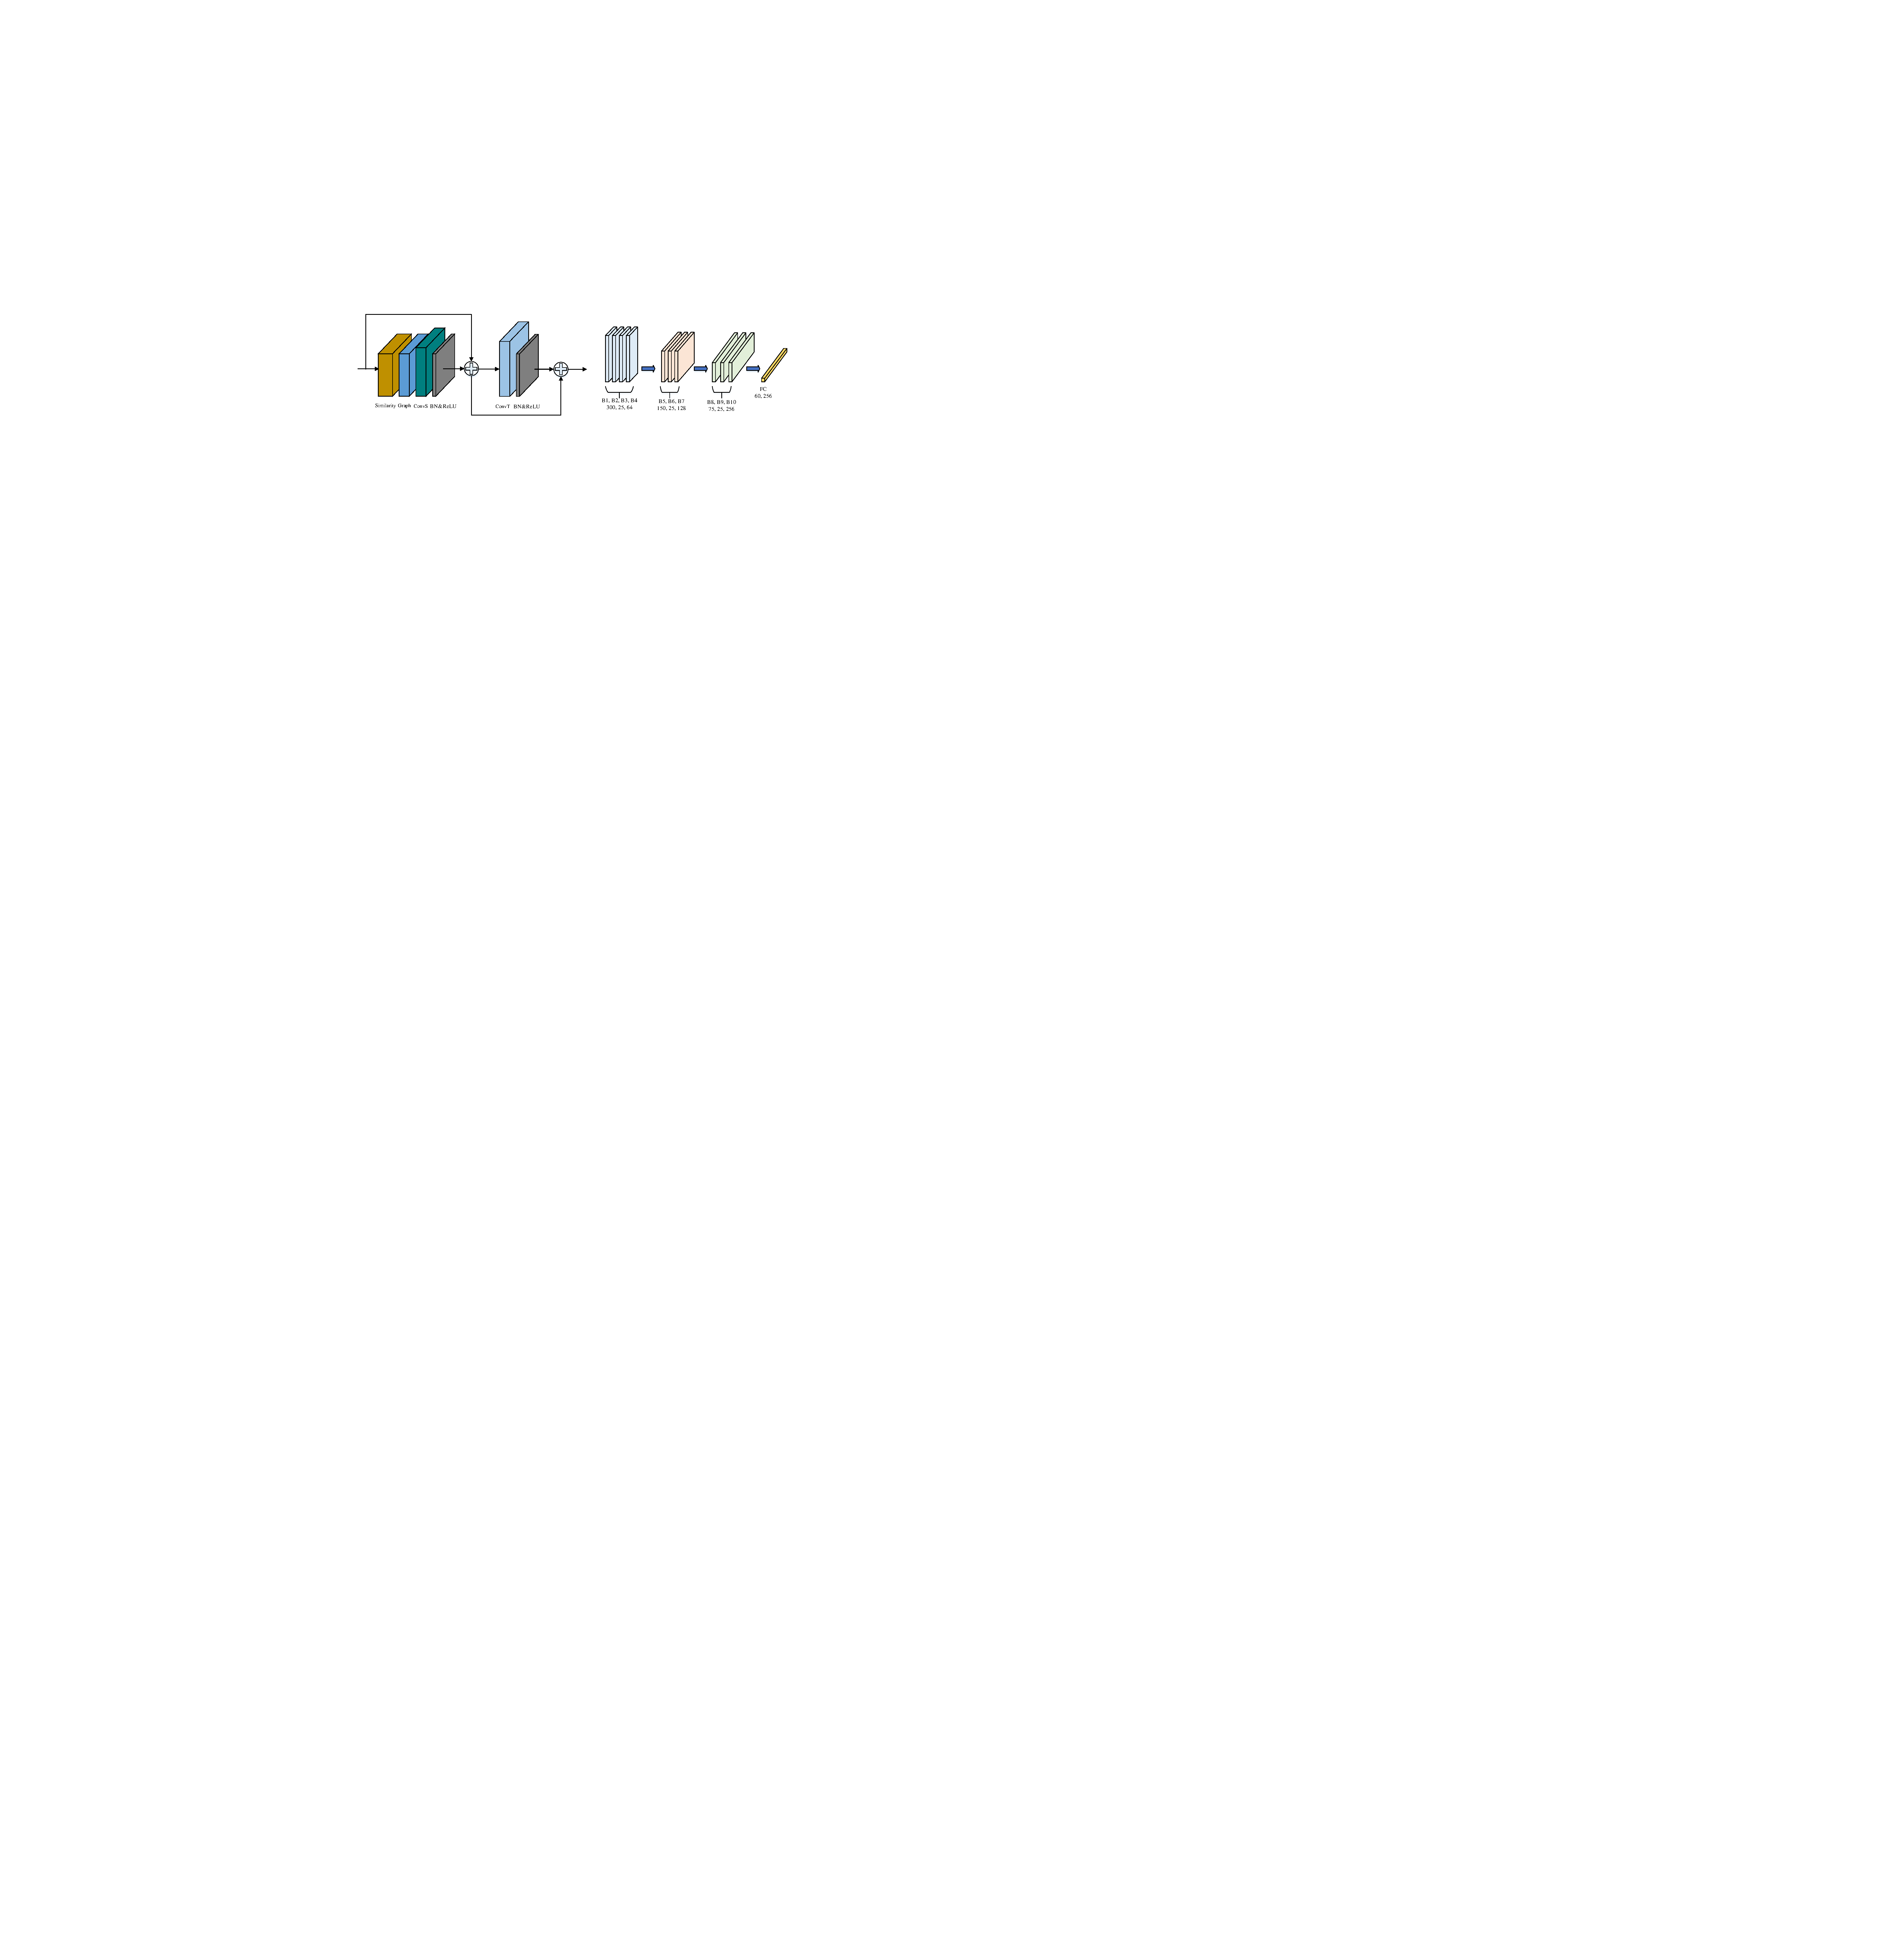
\includegraphics[width=0.42\textwidth]{myfig1.pdf}}
\caption{(a). Structure of the basic convolutional block. ConvS stands for spatial convolution and ConvT stands for temporal convolution. (b). Variance of the feature dimension. There are 25 key joints in human skeleton and 300 skeleton vectors in the original input feature.}\label{myfig1}
\end{figure}

In each layer��s graph computation, three different graphs are embedded: $A_{k}$, $B_{k}$ and $C_{k}$. The first part $A_{k}$ is the static human skeleton graph, the second part $B_{k}$ is a learnable skeleton connection graph and $C_{k}$ is a data-dependent graph generated from self-similarity process. Elements in $B_{k}$ are trained to indicate hidden relationships between joints and bones. Unlike static graph $A_{k}$, $B_{k}$ is dense and sensitive to numerical changes. $C_{k}$ is produced via \eqref{eq1}, where high-dimension tensors' transposition and multiplication are conducted on input feature. $W_{\theta}$ represents similarity coefficient. To sum up, the computation of graph and spatial convolution can be described as \eqref{eq2}. $K_{\nu}$ denotes the neighbour size of the graph computation and is set to 3 in the 2s-AGCN model. The kernel size of spatial convolution��s weight $W_{k}$  is set to 1.
\begin{equation}
C_{k}=softmax(f_{in}^{T}W_{\theta}f_{in})\label{eq1}
\end{equation}
\begin{equation}
f_{out}=\sum_{k}^{k_{\nu}}f_{in}(A_{k}+B_{k}+C_{k})\bigotimes W_{k}\label{eq2}
\end{equation}

Different from $A_{k}$ and $B_{k}$ which are determined before inference, $C_{k}$ relies on input feature, thus needs runtime computing for each prediction. Table.~\ref{tab1} demonstrates the computing cost of self-similarity. The running performance of 2s-AGCN with and without $C_{k}$ are tested on Nvidia V100. At the cost of computing complexity and longer time-delay, $C_{k}$ only elevates prediction accuracy by 0.3\%. From the view of software-hardware co-design, dropping $C_{k}$ graph is a reasonable trade-off for workload reduction.
\begin{table}[htbp]
\caption{$C_{k}$'s influence on 2s-AGCN model. The throughput can be elevated by 29.83\% without $C_{k}$.}
\begin{center}
\begin{tabular}{|c|c|c|c|}
\hline
 &accuracy&throughput&power efficiency \\
\hline
2sAGCN+C&93.70\%&69.38 fps&0.28 fsp/watt \\
\hline
2sAGCNwoC&93.40\%&98.87 fps&0.40 fps/watt \\
\hline
\end{tabular}
\label{tab1}
\end{center}
\end{table}

Following the spatial convolution, temporal convolutional layer is set at the end of each convolutional block. With kernel size of $9\times1$, temporal convolution extracts information from nine skeleton vectors in time order. Despite the insertion of the graph computation, temporal convolution layer in block $l$ can still be seen as the leading neighbour of spatial convolution layer in next block  because graph computation does not change temporal convolutional result along its output-channel dimension, and spatial convolution operates indirectly on temporal convolution's output in block $l+1$ \cite{zhu2020efficient}. For above reasons, the connection shown in Fig.~\ref{myfig2} guides us to conduct coarse-grained pruning on temporal convolutional filters.
\begin{figure}[htbp]
\centerline{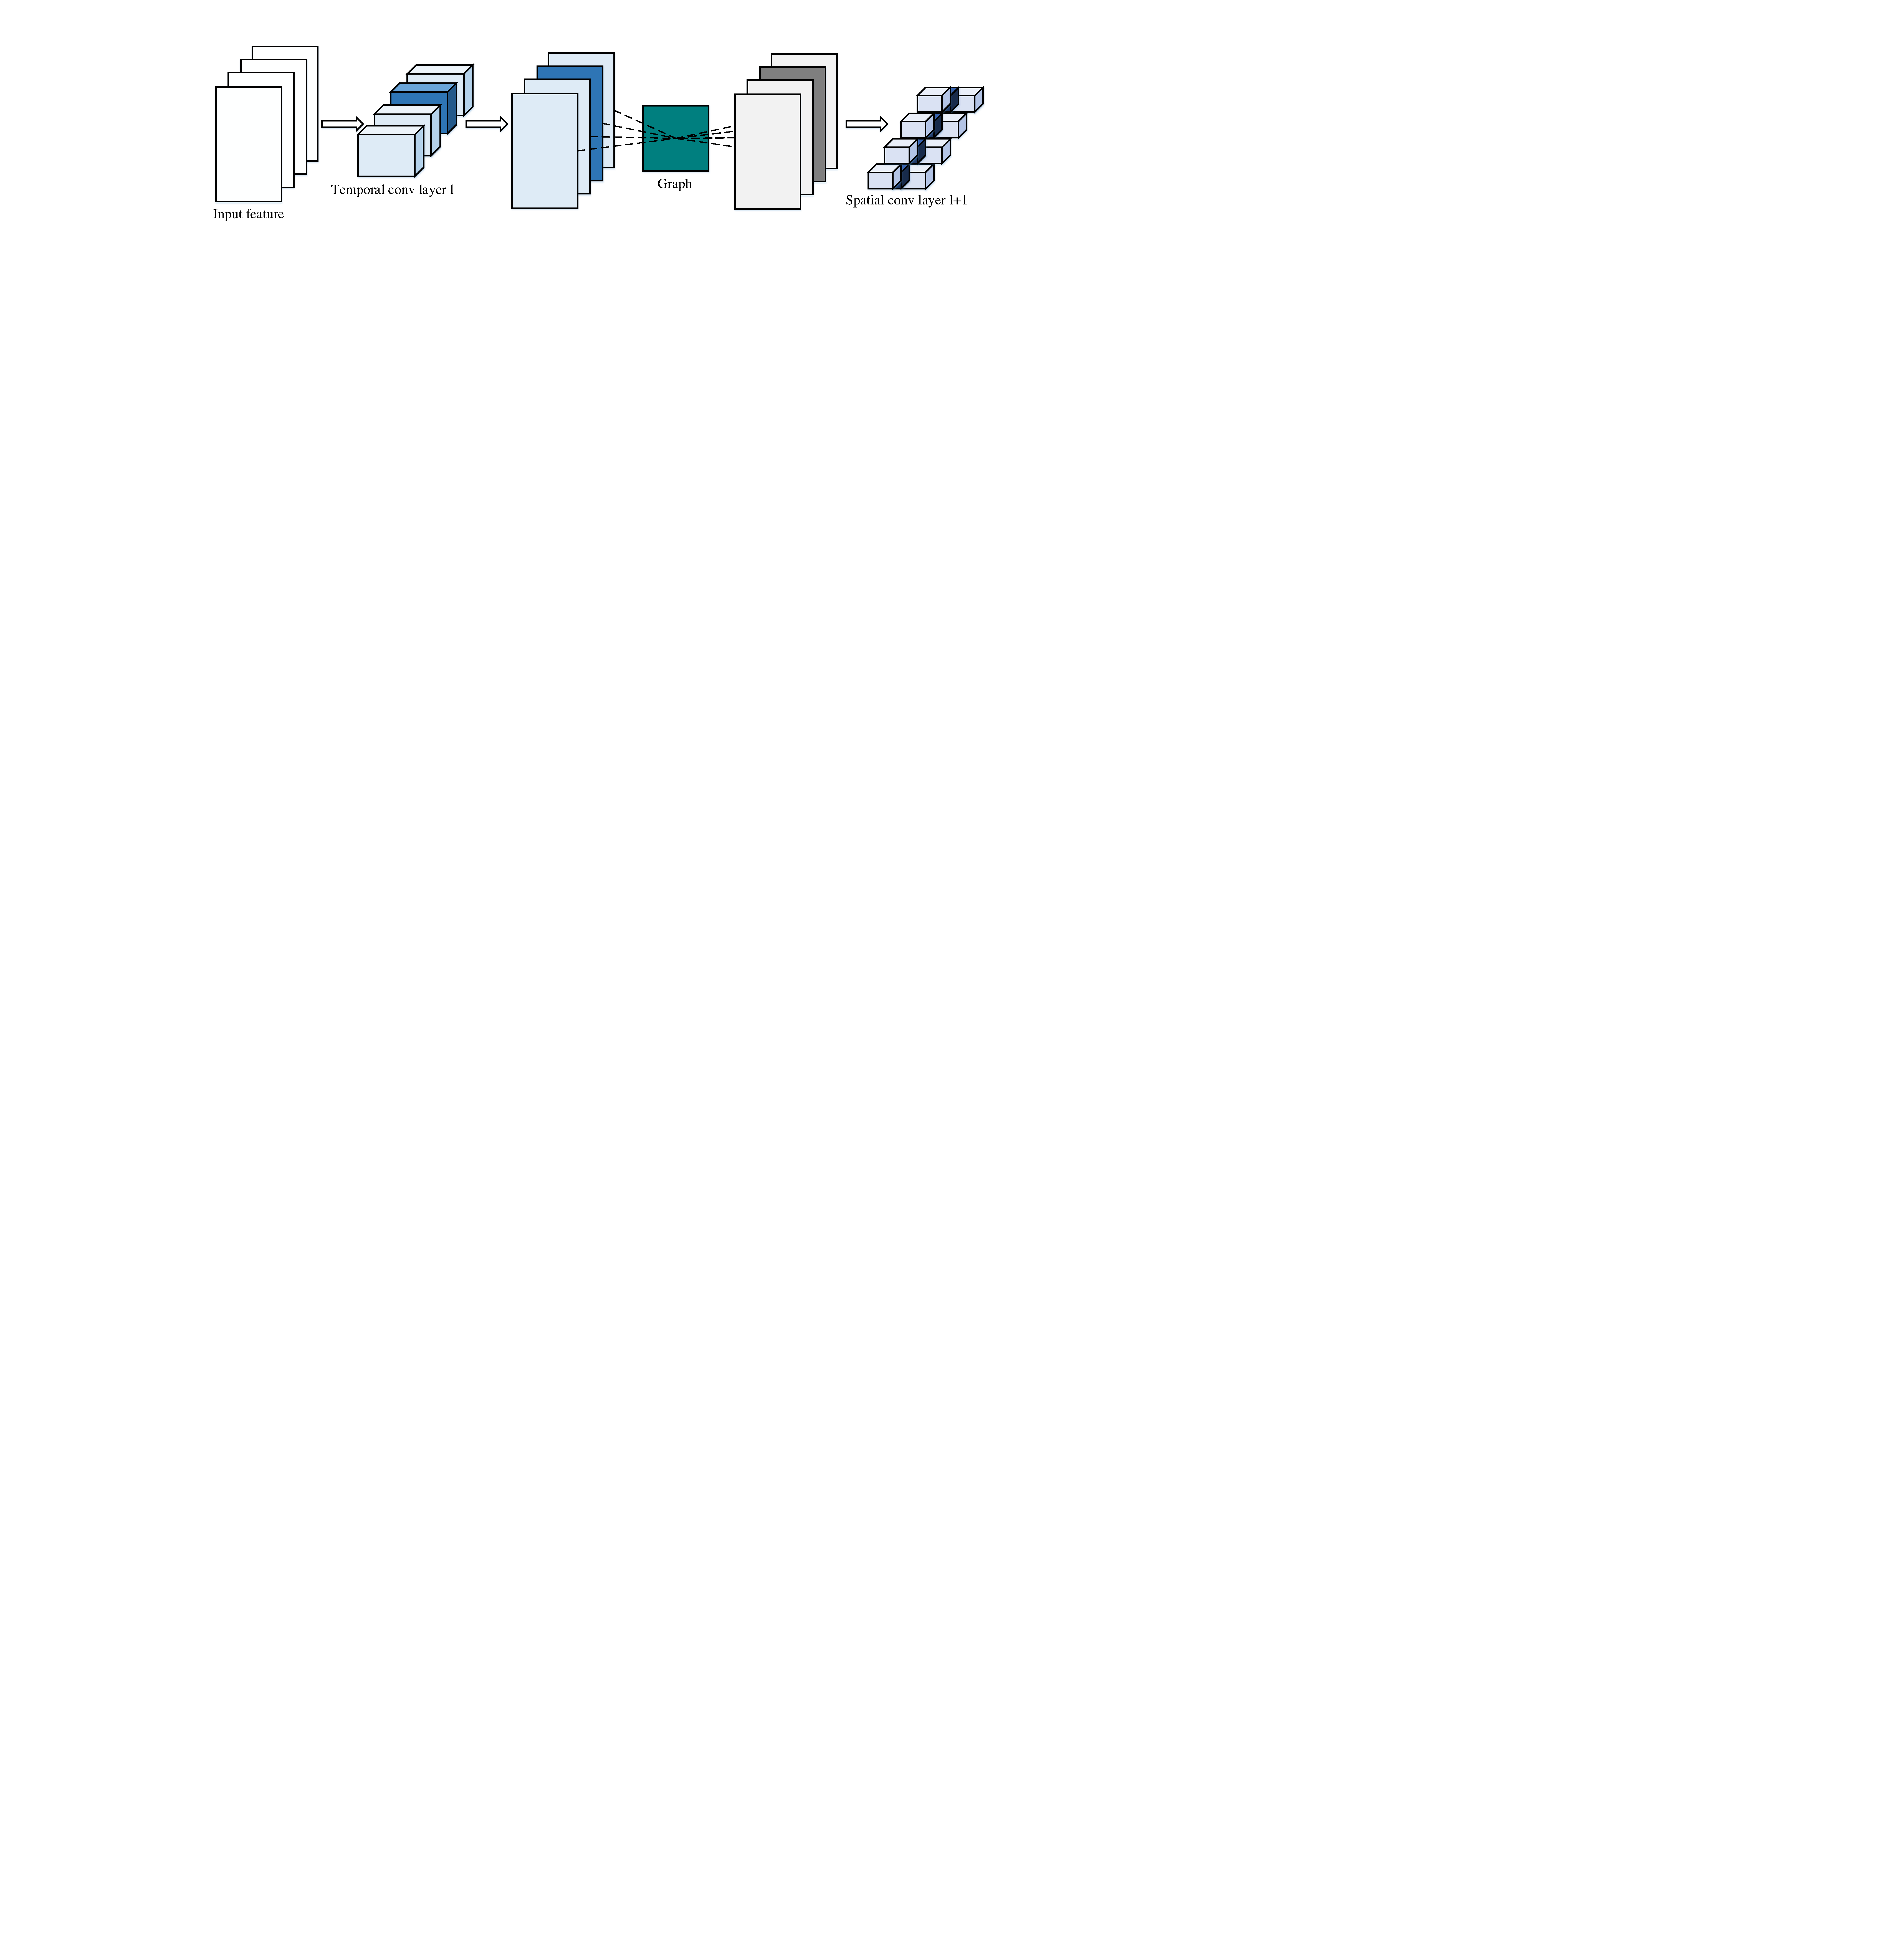
\includegraphics[width=0.42\textwidth]{myfig2.pdf}}
\caption{Temporal convolution��s output channel is the input channel of spatial convolution.}\label{myfig2}
\end{figure}

\section{Related Work}

\textbf{CNNs Accelerators on FPGA.} Works on FPGA-based acceleration of sparse CNNs can be categorized by different pruning granularity levels \cite{zhu2020efficient}: (i) for coarse-grained pruned models, (ii) for fine-grained pruned models, (iii) for mixed-grained pruned models. Zhu et al. \cite{zhu2020efficient} present a zero-skipping dataflow for feature. Although such method raises computing efficiency, zero elements in temporal result still occupy storage resource. Lu et al. \cite{lu2019efficient} propose a weight-oriented dataflow for fine-grained pruned CNNs with little decoding cost. However, our 2s-AGCN model differs from above convolutional workloads in that feature first goes through graph matrix multiplication. Despite this weight-oriented design ignores useless convolutional computation, it cannot skip corresponding graph computation. Li et al. \cite{li2020high} work on PCONV pruning \cite{ma2020pconv}, a mixed-grained method. With weight-stationary dataflow designed on FPGA, Li et al. improve the computing efficiency by 14.7\%~44\%. However, this work still occupies storage space for huge scale of zero data like Lu et al, and its simple hardware structure cannot tackle complex workloads in our task.

\textbf{GCN Accelerators on FPGA.} Many works on accelerating large graph's GCNs based on FPGA are presented in recent time. AWB-GCN \cite{geng2020awb} combines offline software averaging and runtime hardware workloads balancing on several large graph datasets. Zhang et al. \cite{zhang2020hardware} partition input data into smaller segments, then perform graph sparsification and node re-ordering for computation reduction and data locality. Hy-GCN  \cite{yan2020hygcn} splits GCNs workloads into \textit{Aggregation and Combination} phases. Different hardware structures and dataflows are designed for two phases respectively. To sum up, above works focus on: (i) leveraging and expanding graph adjacency matrix��s sparsity, (ii) avoiding irregularity and randomness of data distribution in graph computation, (iii) keeping balanced workloads between PEs or computing phases, via offline and online ways. Unfortunately, graph in skeleton-based GCNs for action recognition models is dense and unchangeable. The data sparsity is embedded in temporal feature and pruned weights, not the graph. Moreover, action recognition GCNs behave not only like CNNs, but also like graph processing, leading to graph-specific design requirements. Therefore, current specialized architectures on CNNs and GCNs cannot efficiently perform target algorithms since they just address one of the two sides.

While there exist many GCNs accelerators on large graph in social media and graph analytics, few works have been proposed to accelerate skeleton-based GCNs for action recognition. ST-GCN, a smaller GCNs model for action recognition, is accelerated by Ding et al. \cite{ding2019fpga} on FPGA. Their work falls short on more complex action recognition GCNs for: (i) they only apply quantization on model, does not prune or optimize ST-GCN; (ii) Ding et al. compress human skeleton graph into CSC format, while skeleton relationship matrix in 2s-AGCN is dense; (iii) their hardware design is established on sparse matrix-vector multiplication (SpMV) units for sparse skeleton matrix. Data sparsity in feature is not thoroughly utilized in their work; (iv) its single-PE design does not meet the performance requirement of expected application scenario.

\section{Methodology}
This section introduces our hybrid pruning method for action recognition GCNs. The dataflow reorganization, coarse-grained and fine-grained pruning on temporal convolution are described respectively.
\subsection{Dataflow Reorganization}
After clipping self-similarity graph, the computing flow between graph and spatial convolution can be further summarized as \eqref{eq3}, where $G_{k}$ denotes $A_{k}+B_{k}$ from \eqref{eq2}. The computing order is first high-dimensional matrix multiplication with $G_{k}$, then the spatial convolution of $W_{k}$ and finally the result merging of three loops. In this dataflow, common pruning methods only functions in second phase but cannot optimize the graph computation, which occupies 49.83\% of total workloads in \eqref{eq3}.

\begin{equation}
f_{out}=\sum_{k}^{k_{\nu}}f_{in}G_{k}\bigotimes W_{k}\label{eq3}
\end{equation}

To better analyse the dataflow, we extract first two phases and its output \textit{X}. A pixel can be described as $X(h, w, oc)$, where \textit{h, w, oc} represent height, width and output-channel coordinates respectively. \eqref{eq4} can then be deduced from \eqref{eq3} and \textit{ic} is the acronym of input channel. Under the commutative law of multiplication, \eqref{eq4} therefore is transformed into \eqref{eq5}. By reorganizing the computing order between graph phase and convolution phase, an opportunity for graph-skipping pruning is offered here. If the parameter element $W(1, 1, i, oc)$ is pruned to zero, the graph matrix multiplication in current output channel can be ignored. Further, if we set all convolutional parameters in \textit{i} input channel as zero, then all graph computation can be skipped in current loops. The dataflow reorganization is then proposed when we apply above method to three loops in \eqref{eq3}. Unlike conventional structure pruning method which drops different channels on filters, weights in specific input channels are all set as zero on every spatial filter in current convolutional blocks. In this way, not only the convolution workload is reduced, but also the graph computation is skipped.

\begin{small}
\begin{equation}
X(h, w, oc)=\sum_{i=1}^{ic}(\sum_{p=1}^{25}f_{in}(h, p, i)\times G(p, w))\times W(1, 1, i, oc)\label{eq4}
\end{equation}
\end{small}
\begin{small}

\begin{equation}
X(h, w, oc)=\sum_{i=1}^{ic}(\sum_{p=1}^{25}G(p, w)\times f_{in}(h, p, i)
\times W(1, 1, i, oc))\label{eq5}
\end{equation}
\end{small}

Since the graph-skipping strategy has been determined by dataflow reorganization, the next step is choosing the input channel to be pruned. Like other deep neural networks (DNN), features between convolutional layers are sparse and useful elements are unevenly distributed. Fig.~\ref{myfig3} demonstrates the data sparsity and distribution of 2s-AGCN model. Based on the observation that unstructured pruning method drops weight element with relatively small absolute value, we cut off the input channels which have least averaging absolute data. In this way, data reorganization prunes spatial convolutional weight and skips both graph and convolution computation.
\begin{figure}[htbp]
\centerline{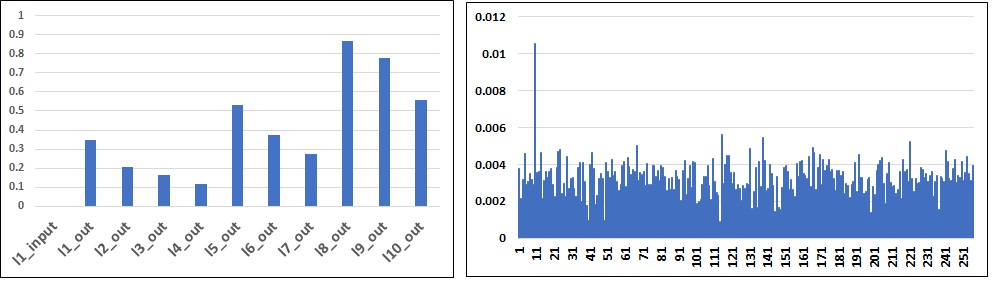
\includegraphics[width=0.45\textwidth]{myfig3.png}}
\caption{The demonstration of data sparsity and distribution of 2s-AGCN model. The left figure shows data sparsity of each block's output feature. The right one is the averaging absolution of block 8��s output along channel, where \textit{x} axis denotes channel and \textit{y} axis denotes averaging absolute value.}\label{myfig3}
\end{figure}
\subsection{Mixed-grained Pruning Method}
Dataflow reorganization leads to features in specific channels being not computed for specific channels are pruned on filters. The coarse-grained method prunes corresponding temporal filters via connections in Fig.~\ref{myfig3} with no extra accuracy loss. Moreover, this neighbour connection is hardware-friendly for that the number of pruned channels in spatial filters equals the number of pruned filters in temporal convolution. This inherent feature supports a balanced layer-pipelined architecture.
\begin{figure}[htbp]
\centerline{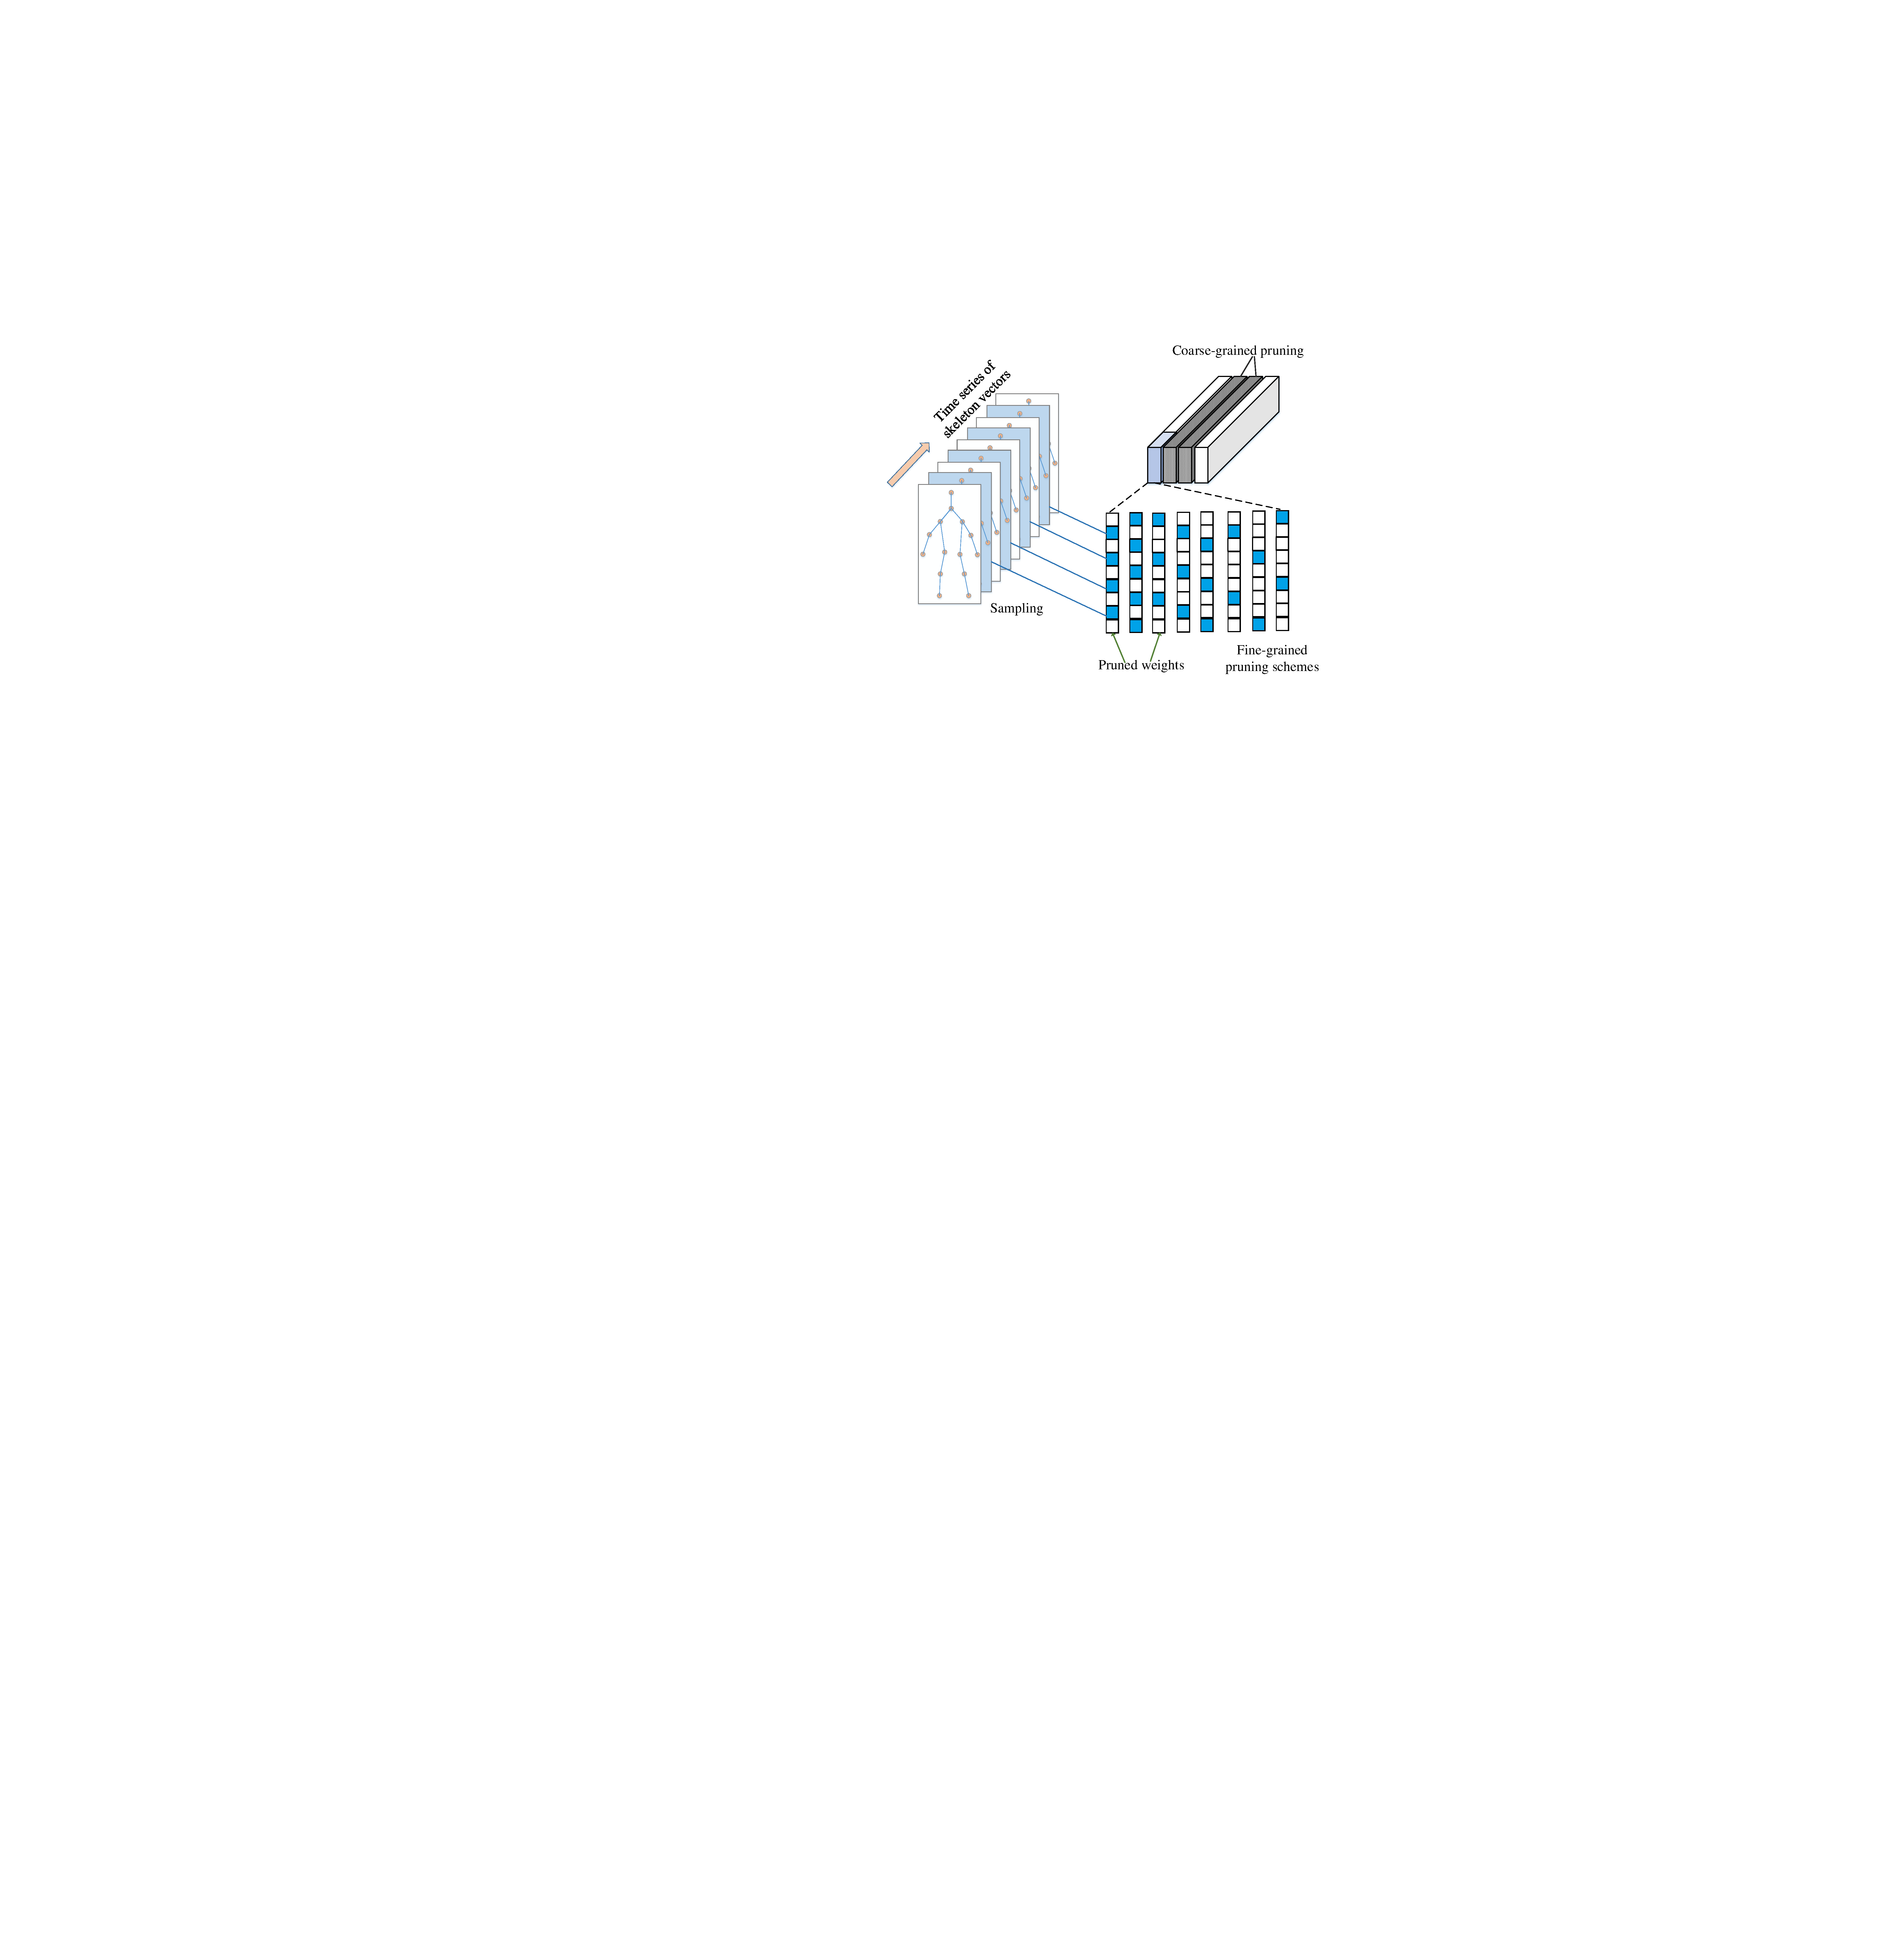
\includegraphics[width=0.32\textwidth]{myfig4.pdf}}
\caption{The illustration of fine-grained pruning on temporal convolution. White elements are pruned while blue ones are kept. Every 9x1 kernel performs on time series of skeleton vectors, and the blue vectors are sampled by first pruning scheme.}\label{myfig4}
\end{figure}
\begin{figure*}[htbp]
\centerline{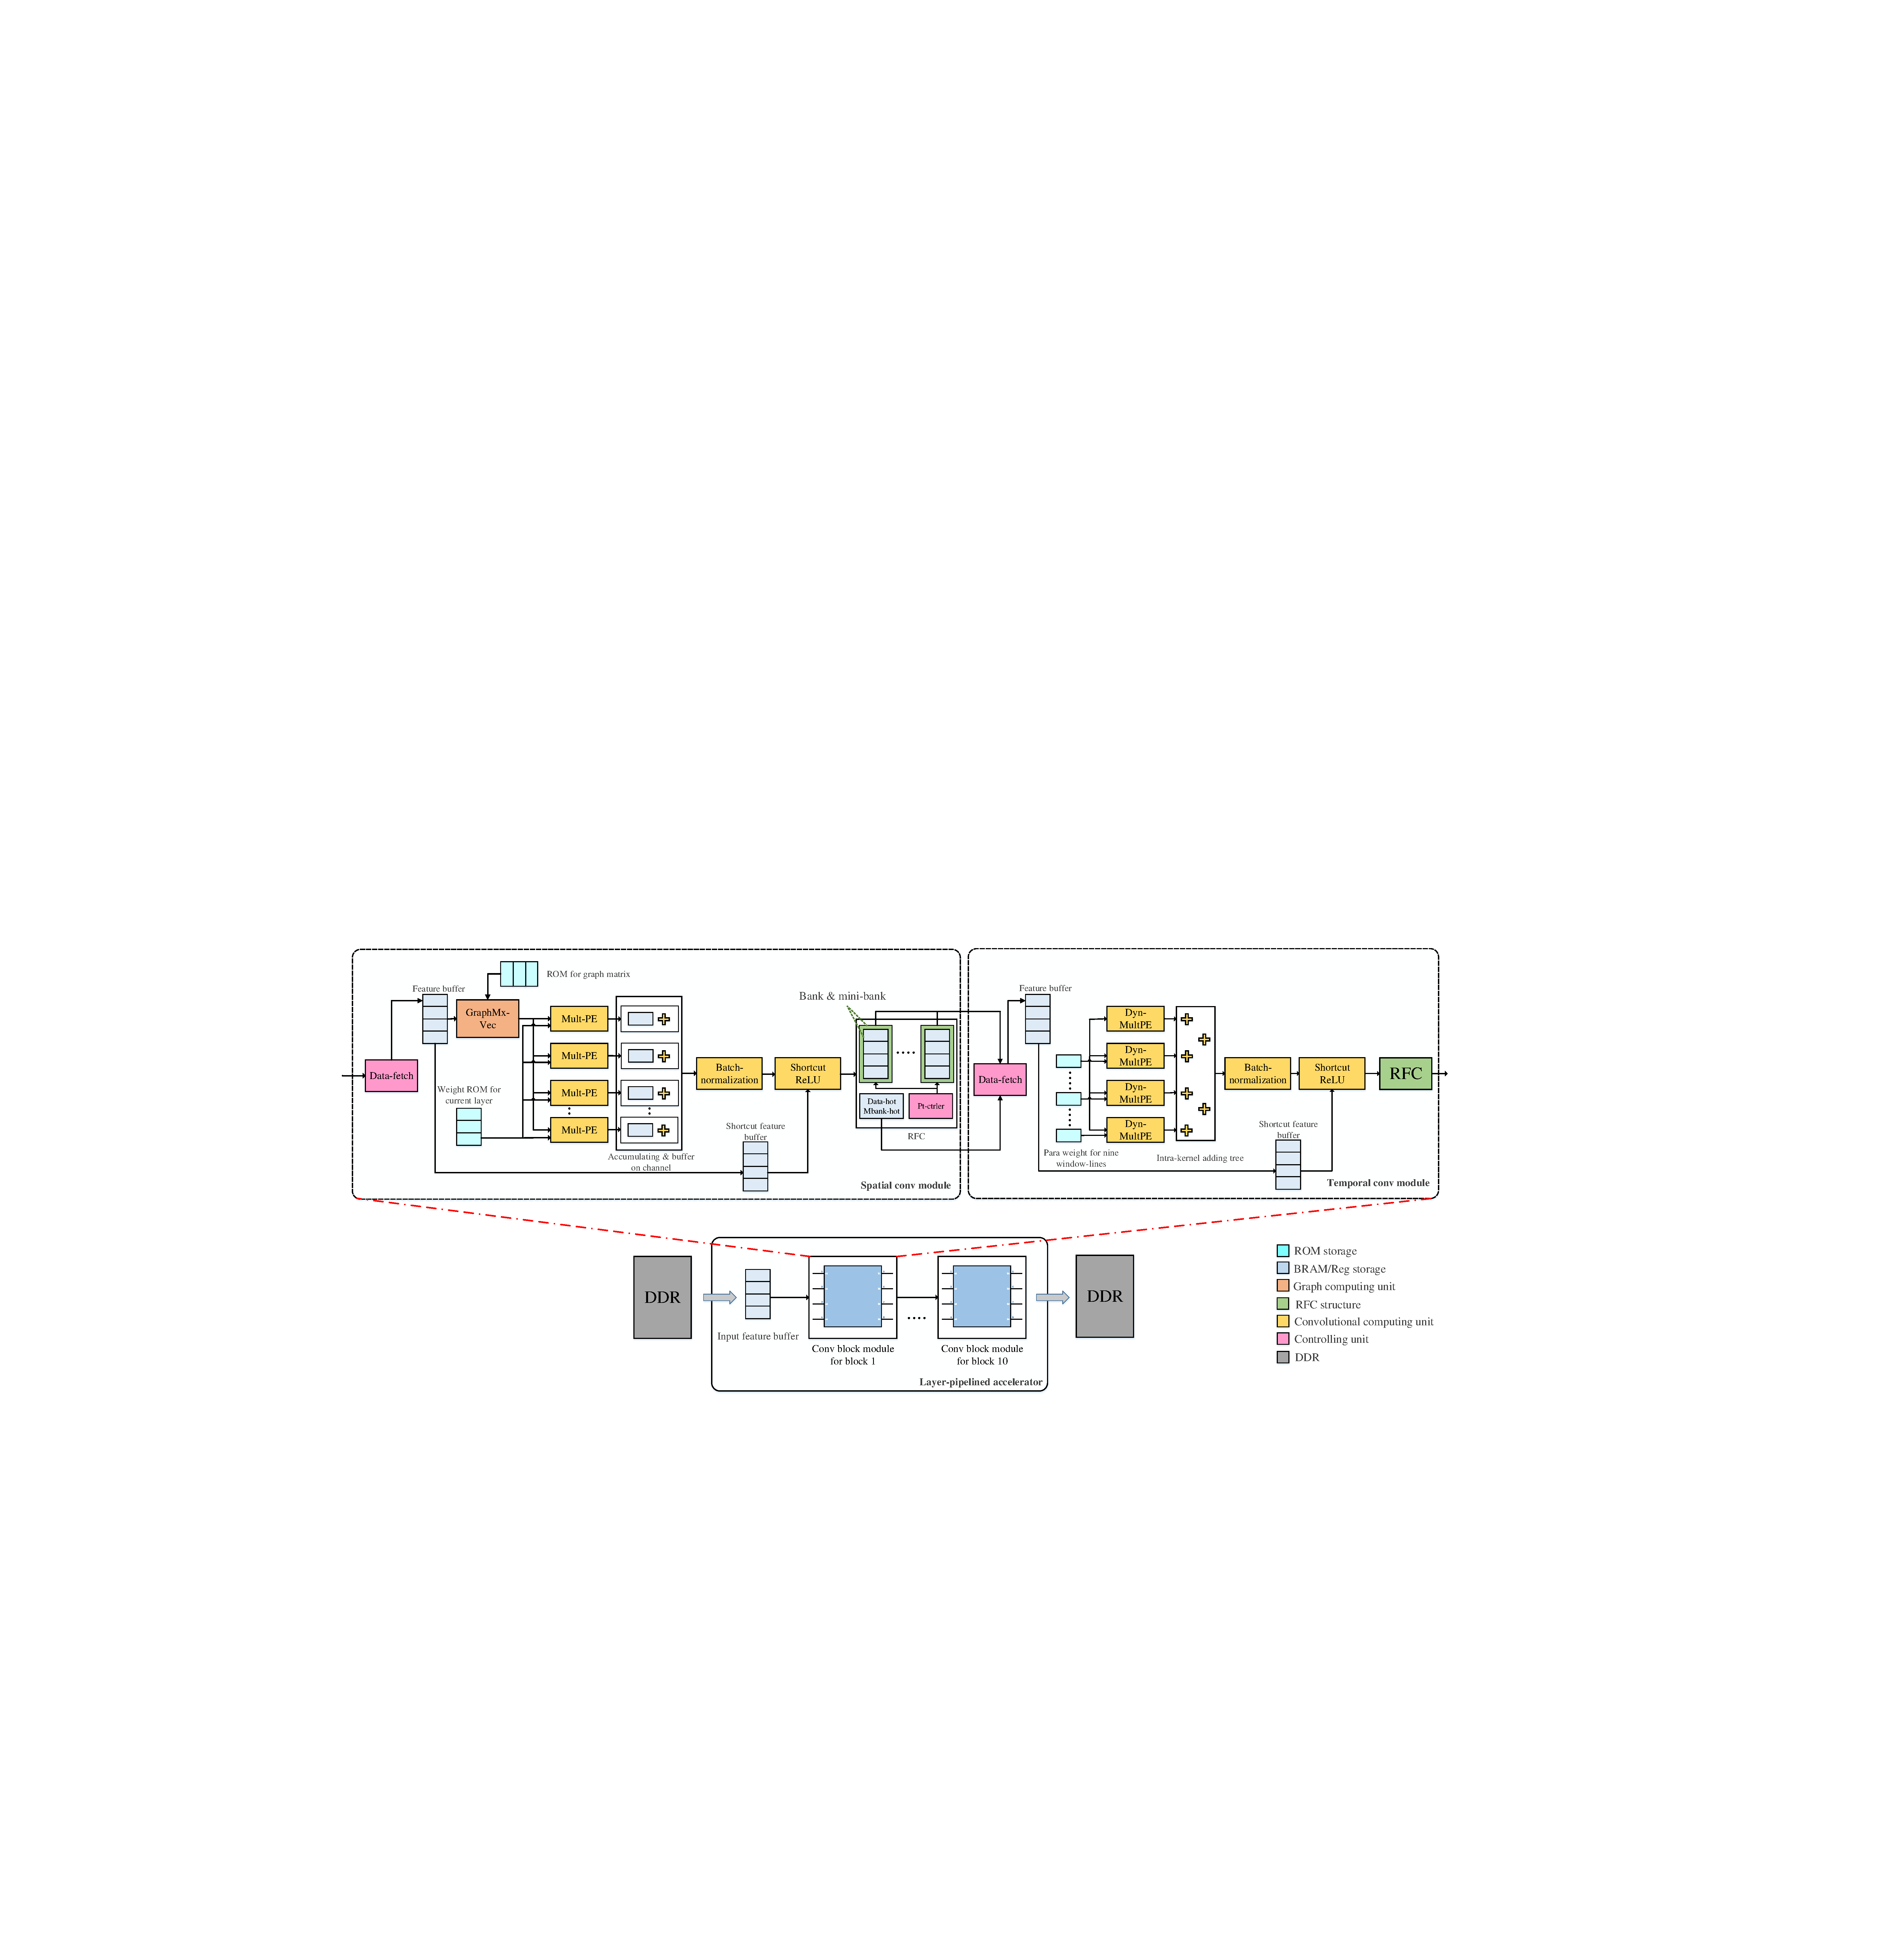
\includegraphics[width=0.82\textwidth]{myfig5.pdf}}
\caption{The demonstration of overall architecture.}\label{myfig5}
\end{figure*}

Coarse-grained pruning can provide 49.83\%-88.96\% compression ratio on temporal filters, depends on the pruning scheme in data organization phase. To further prune temporal convolutional weights, fine-grained pruning is proposed. The point of fine-grained method is that in temporal convolution, zero weight means not sampling current vectors in time order. Fig.~\ref{myfig4} demonstrates details of sampling-like fine-grained pruning method. Several pruning schemes with different intervals and offsets are conducted on filters recurrently. By this means, the pruning scheme design is turned into a sampling problem. We can simulate various sampling schemes on filters, with different sampling frequencies and phases being represented by intervals and offsets. Experiments show that with proper pruning scheme, our fine-grained method can keep accuracy as well as discarding unimportant weight.


Conventional unstructured pruning methods randomly drop the weight elements with least absolute value, which are expensive and unbalanced on hardware. However, with determined cavity schemes, our fine-grained pruned model can be indicated by structured weight together with masks. Furthermore, we guarantee the balancing distribution of reserved weight by controlling start-points of different sampling patterns. Like Fig.~\ref{myfig4} shows, in a loop of eight different pruning modes, weight elements in every position of kernels are evenly kept by two or three times. Also, compression ratio can be adjusted via fine-grained pruning design.

\section{Architecture}

This section introduces the detailed architecture of our accelerator, where all pruned convolutional blocks are mapped on chip.

\emph{Overview}: Fig.~\ref{myfig5} depicts the overall design of our layer-pipelined architecture. In our layer-pipelined design, conv block module for each block constitutes the whole architecture. To be more detailed, one spatial conv module (SCM) and one temporal conv module (TCM) are included in a conv block module. For proposed pruning method reduces model size, all convolutional parameters and graph are stored in ROM storage. Moreover, runtime sparse feature compression module (RFC) functions at the junctions of different layers to compact and store temporal results.

\subsection{Spatial conv module}
The main task of SCM is performing graph computation and pruned spatial convolution2. Feature buffer stores the extended feature vectors, which are decoded in Data-fetch part. Data-fetch controls the address of data-loading and decodes compact feature into sparse form, which is convenient to compute. The decoding process will be explained later. Sparse feature will first multiply with graph vectors, and then conduct convolution with non-zero weight in Mult-PE. Pruned channels are skipped and multiplication results are summed up in accumulating buffer on output channel. After batch-normalization operation, dataflow merges with original input activation, which is stored in shortcut feature buffer. ReLU function is combined with encoding function parts, where sparse data is compressed into compact format again.

In order to combine graph computation and pruned convolution workloads, dataflow is organized as Fig.~\ref{myfig6} shows. A line in feature buffer caches 25 data from feature, and the depth of the buffer is varied to store all data in one row of feature tensor. Depth equals the number of input channels in different blocks. When computing, feature buffer offers one line of original feature data. After computation with one column vector of graph, this feature vector generates one valid element $X(h, w, oc)$ in \eqref{eq4}. Afterwards, feature buffer provides data in next cache line, which continues to produce $X(h, w, oc+1)$. Following this mode, when all output elements on current output channel are computed, feature buffer returns to the first line and graph ROM switches to the next column vectors to prepare for $X(h, w+1, 0: N_oc)$. When the workload of one row feature tensor is finished, feature buffer receives next row of tensor to start a new sub-loop. Algorithm 1 depicts the whole loop operation. In this way, feature  is produced in a channel-first order. To be noticed that our dataflow reorganization method essentially abandons feature data on specific channels, so we skip corresponding workloads by not loading them to data-fetch module.
\begin{figure}[htbp]
\centerline{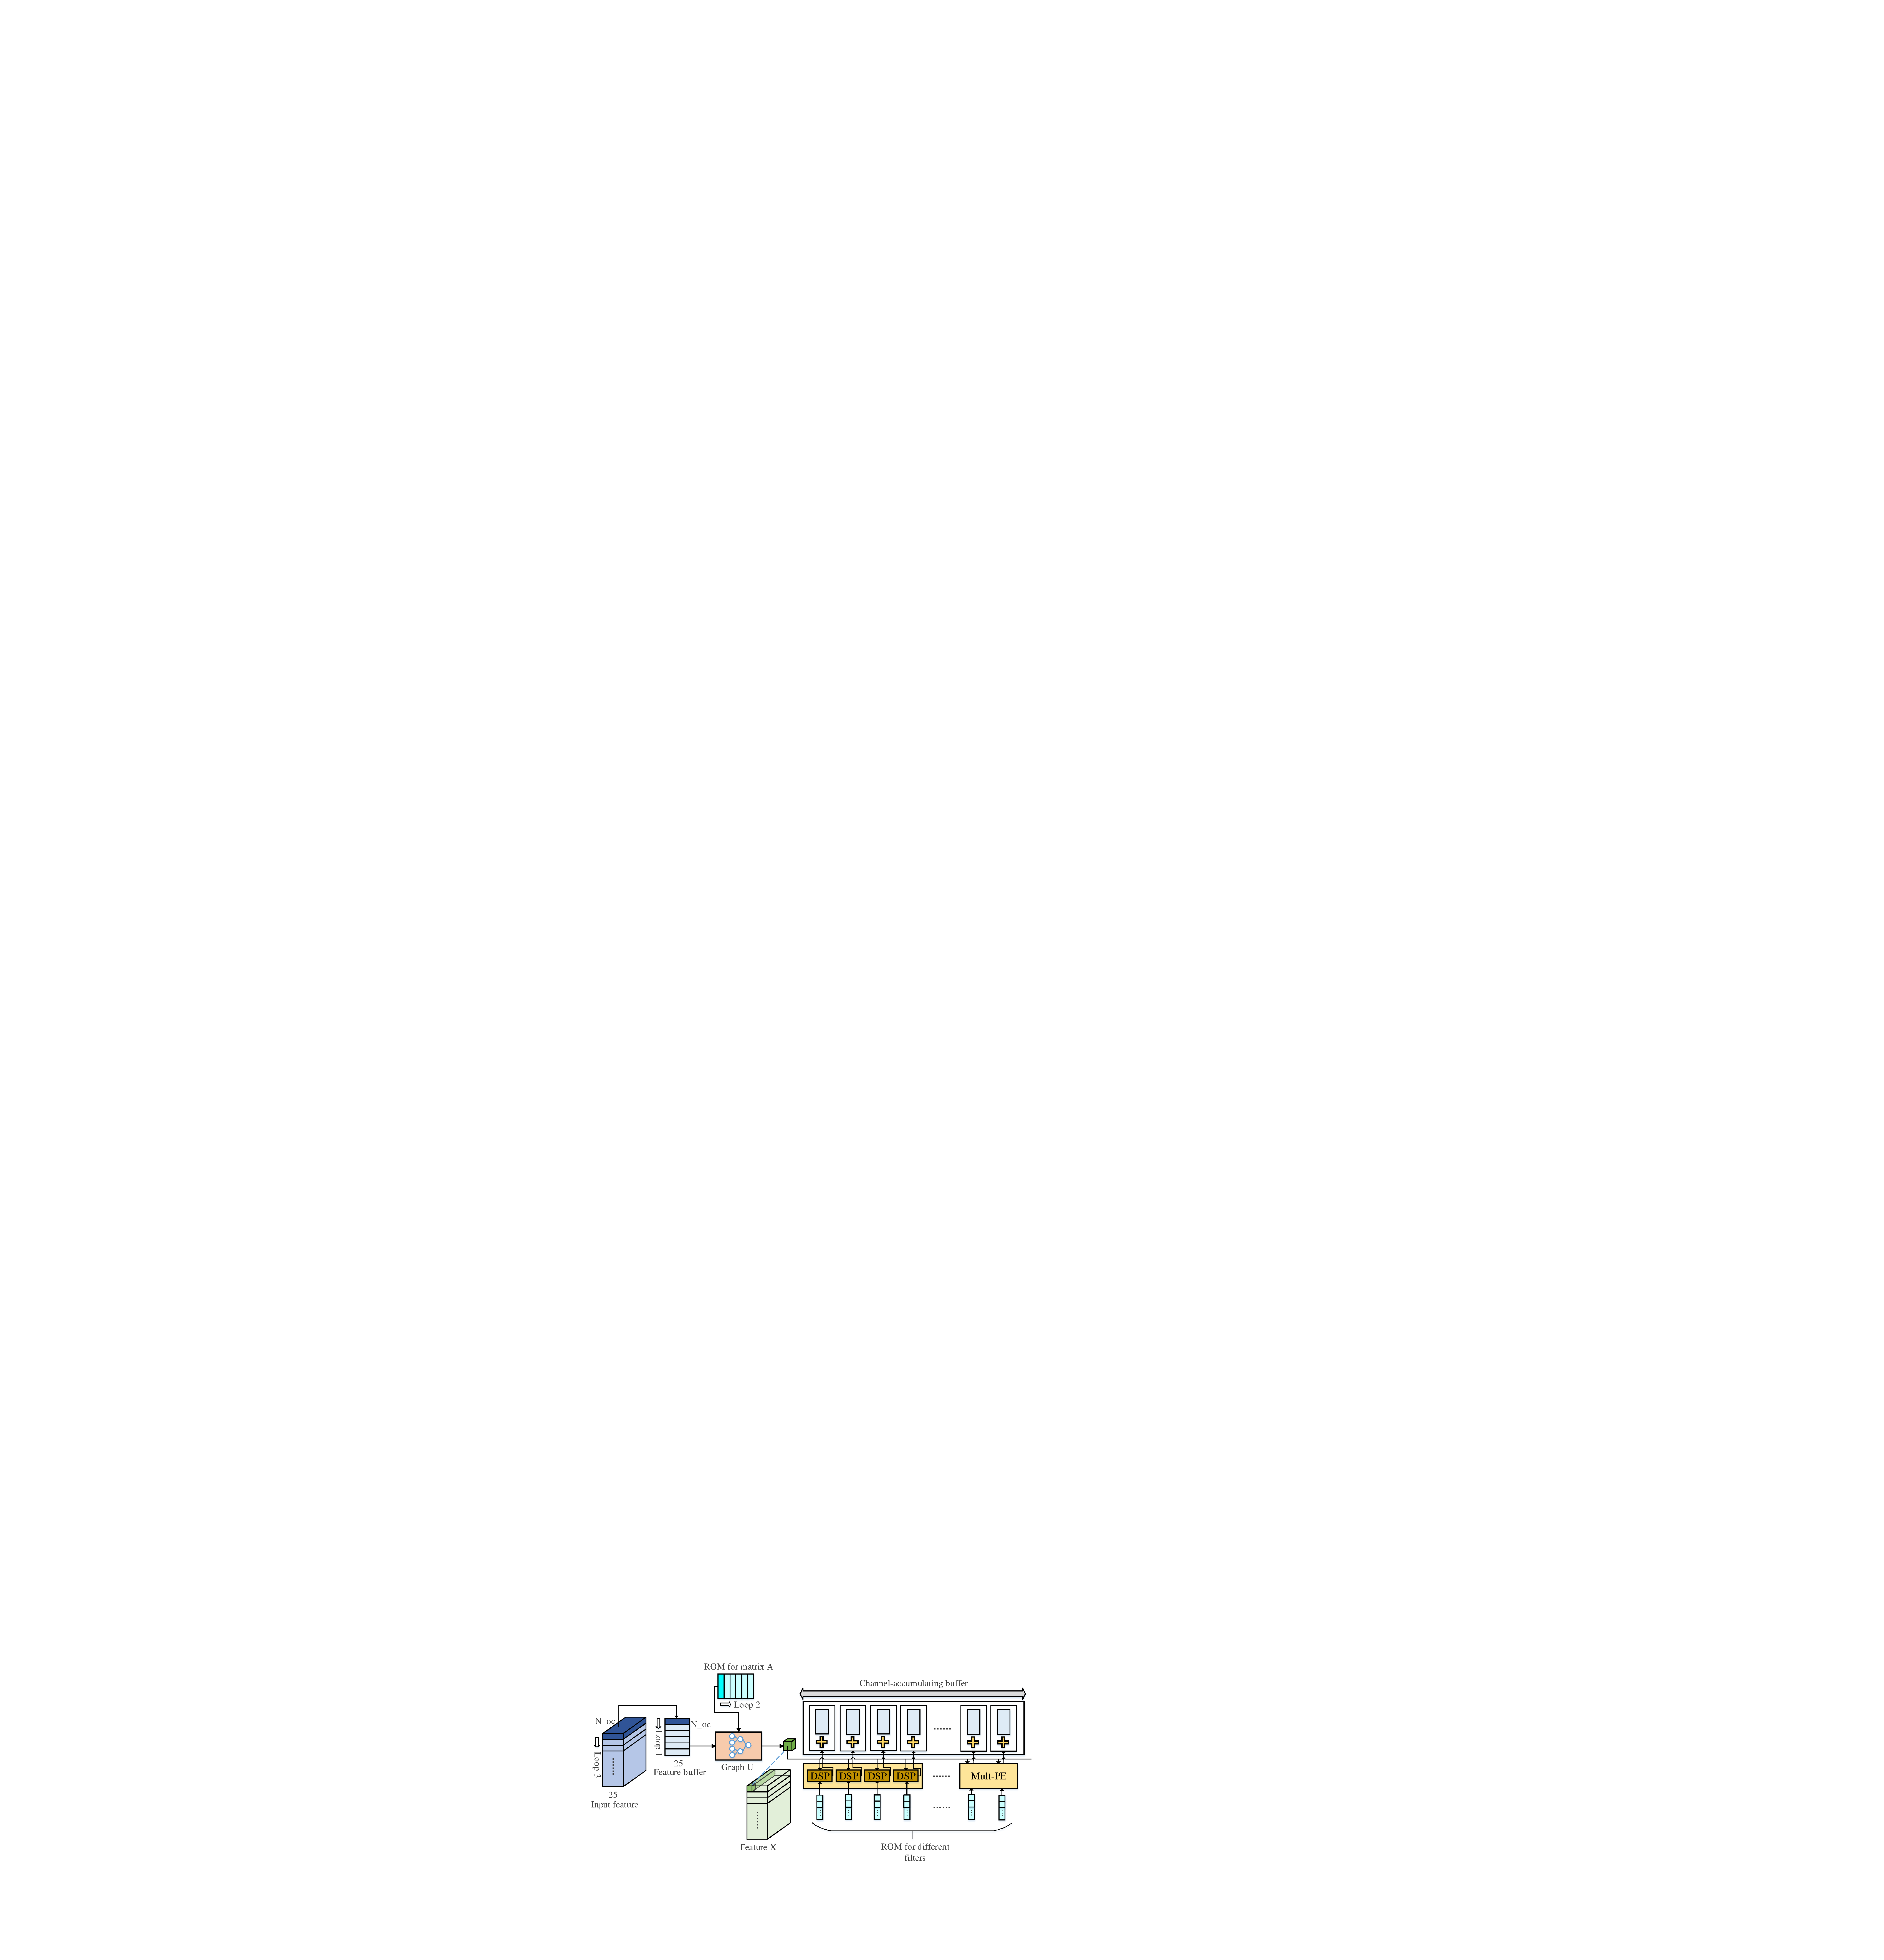
\includegraphics[width=0.42\textwidth]{myfig6.pdf}}
\caption{Illustration of SCM dataflow organization.}\label{myfig6}
\end{figure}
Feature element is broadcast to all Mult-PEs. In the same channel-first order, weight ROM sends different filters' parameters into different computing units. To cooperate with the pruned model and feature-loading-skipping mechanism, only non-zero elements in filters are stored in ROM with original order. Each Mult-PEs includes four DSPs, and by adjusting the number of Mult-PE, our design can fit into different layers. Results from parallel Mult-PEs are accumulated and buffered on channel direction as well. When the sum counter reaches the number of valid channels, current data will be transferred into post-processing modules.

\subsection{Temporal conv module}
TCM is designed to accelerate temporal convolution workloads, whose kernel size is $9\times1$. Fig.~\ref{myfig7} shows the detailed information of TCM. Similarly, feature buffer stores decoded data from data-fetch. However, feature buffer��s size is changed to match the kernel size. The width is turned from 25-data into 9-data, and the depth is tuned to be able to hold an $9\times25\times in_c$ area of feature tensor. Additionally, the one-hot code of current feature is sent from data-fetch to feature hot storage as well. Based on mix-grained pruning method, a weight-static workflow is presented in TCM. Firstly, unpruned data together with its masks is stored on chip. Depicted in Fig.~\ref{myfig4}, several balanced fine-grained pruning schemes are conducted on leftover filters in recurrent ways, which provides an opportunity to store effective weight and mask with regularity. One temporal filter is divided into several $1\times 1\times 16$ sub-filters, thus, temporal convolutional parameters can fold into sub-filters format and then be stored in a recurrent mode. Secondary, computing units Dyn-MultPEs are put across input channel and parallelizes on filter's rows. There are two reasons: i) This parallel scheme can directly skip the abandoned filters in coarse-grained pruning, ii) Each row of sub-filters is taken by one Dyn-MultPE, with each function part handling one row of weight tensor. In this way, one Dyn-MultPE only needs to process four or six valid weights with static cavity mask in one sub-filter. This design furthermore eliminates data irregularity and reduces the hardware cost of intra-PE dynamic data scheduling.

\begin{figure}[htbp]
\centerline{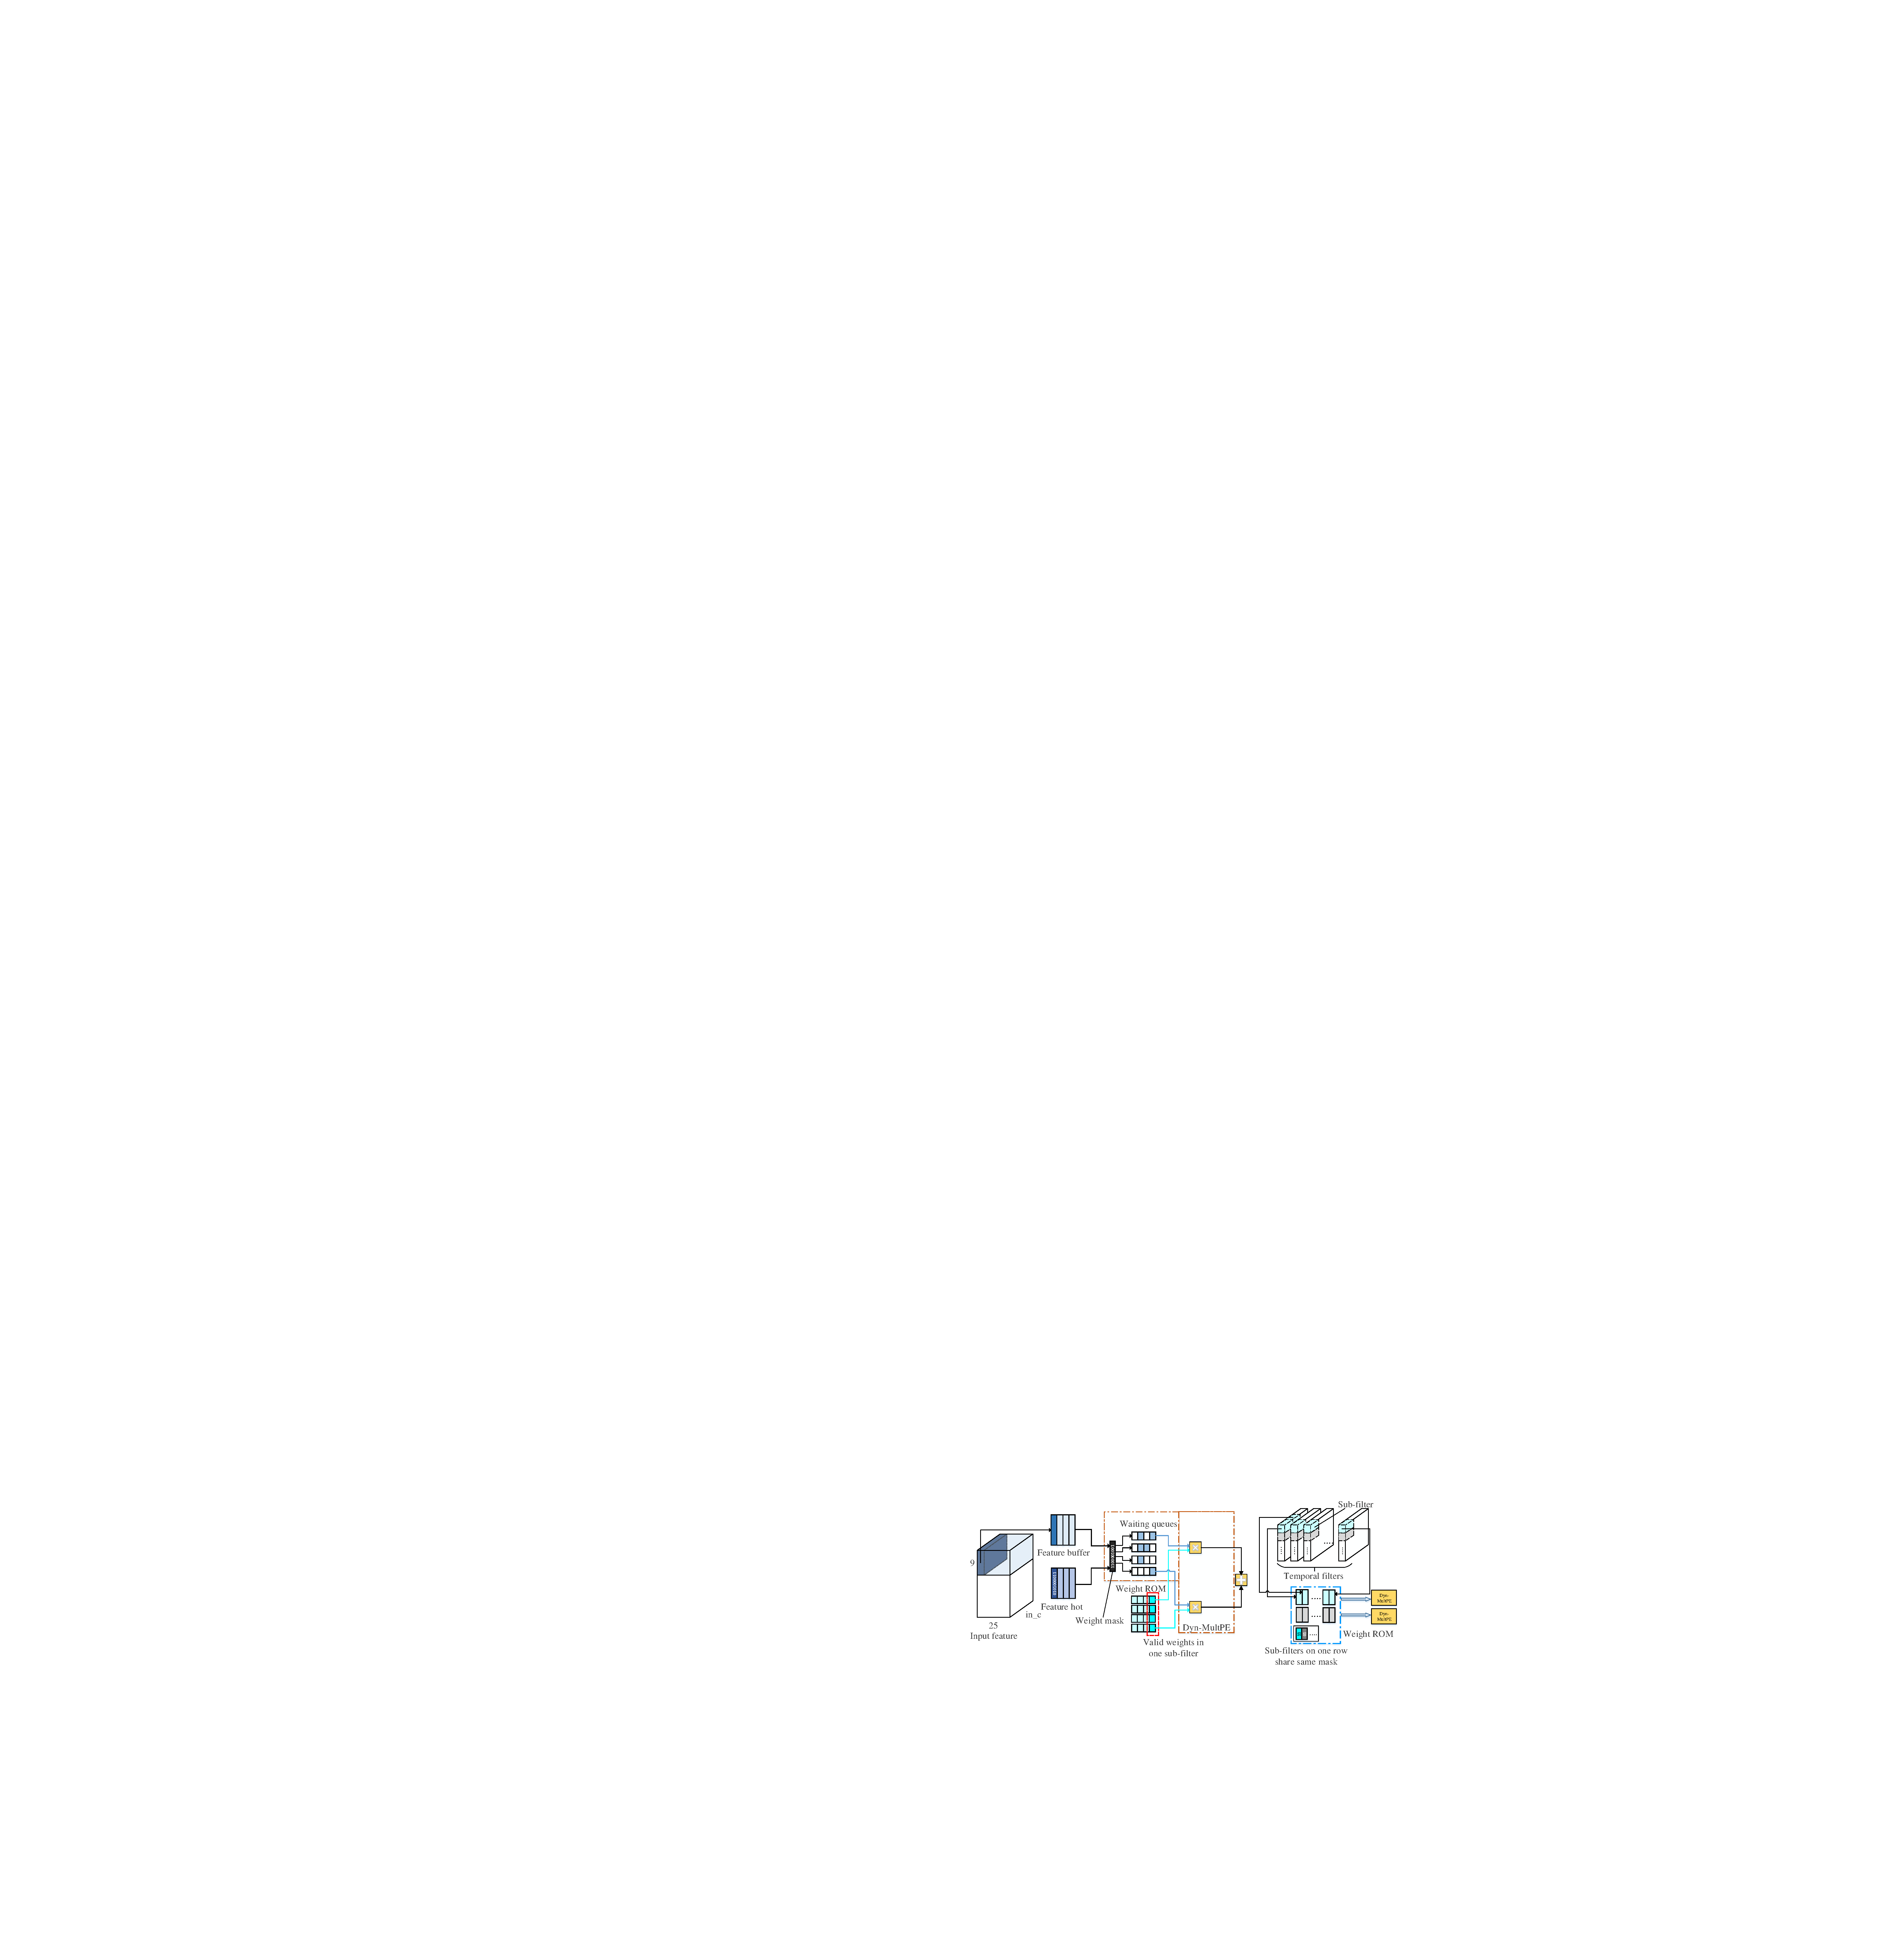
\includegraphics[width=0.42\textwidth]{myfig7.pdf}}
\caption{Illustration of TCM's dataflow.}\label{myfig7}
\end{figure}
Shown in Fig.~\ref{myfig7}, one row of a sub-filter is assigned to a Dyn-MultPE, which includes four or six waiting queues and several DSPs. Logic and operantion is performed first on weight mask and feature mask to skip the zero-feature and dropped weights. Then, valid feature enters one waiting queue, which is bonded to a non-zero weight in the sub-filter. Although weights pruning is balanced, zero-distribution in feature is unpredictable. To decrease the use of DSPs and raise working efficiency of computing resource, dynamic data scheduling is designed by dispatching data from different waiting lines to DSPs. Because multiplication in a Dyn-MultPE represents computation inside one temporal filter, so the results are summed up and afterwards sent to the adder-tree. While dynamic data scheduling has advantages on saving DSP resource, it may increase the working delay at workloads-intensive cases. Taking both delay and efficiency into consideration, we propose the method to estimate the number of needed DSPs based on offline feature sparsity in \eqref{eq5}. With the help of recurrent fine-grained pruning and statistic sparsity, we calculate the expectation of valid computation in one sub-filter and use it to guide the DSP occupation.
\subsection{Runtime sparse feature compress}
Despite layer-pipelined architecture poses great advantages on throughput, it having to store massive temporal computing results for shortcut task. The motivation of our runtime sparse feature compress (RFC) is to decrease on-chip storage utilization by compacting zero feature data.

\textbf{Encoding:} RFC contains encoding parts, compact storage and decoding parts. Encoding process is combined with ReLU while decode is embed in data-fetch module in TCM and SCM. The whole structure of RFC is displayed in Fig.~\ref{myfig8}. At first, one feature vector is divided into several banks across channels. The width of each bank is 16 data-wise. ReLU function parts perform on banks, providing activation and one 16-bit hot code, which denotes the positive/zero value of ReLU results. Moreover, valid elements are gathered at higher bits while unused bits are padded with zero. After that, mini-bank-hot code (mbhot) is generated according to the number of non-zero data in current bank. Mbhot indicates which mini-banks are used in the bank storage. Encoding parts work in pipeline and during several working cycles, the whole vector is finally turned into compact format. Instead of compressing one vector as whole, we lower the encoding cost by setting bank as the finest grain of ReLU and encoding process.

\begin{figure}[htbp]
\centerline{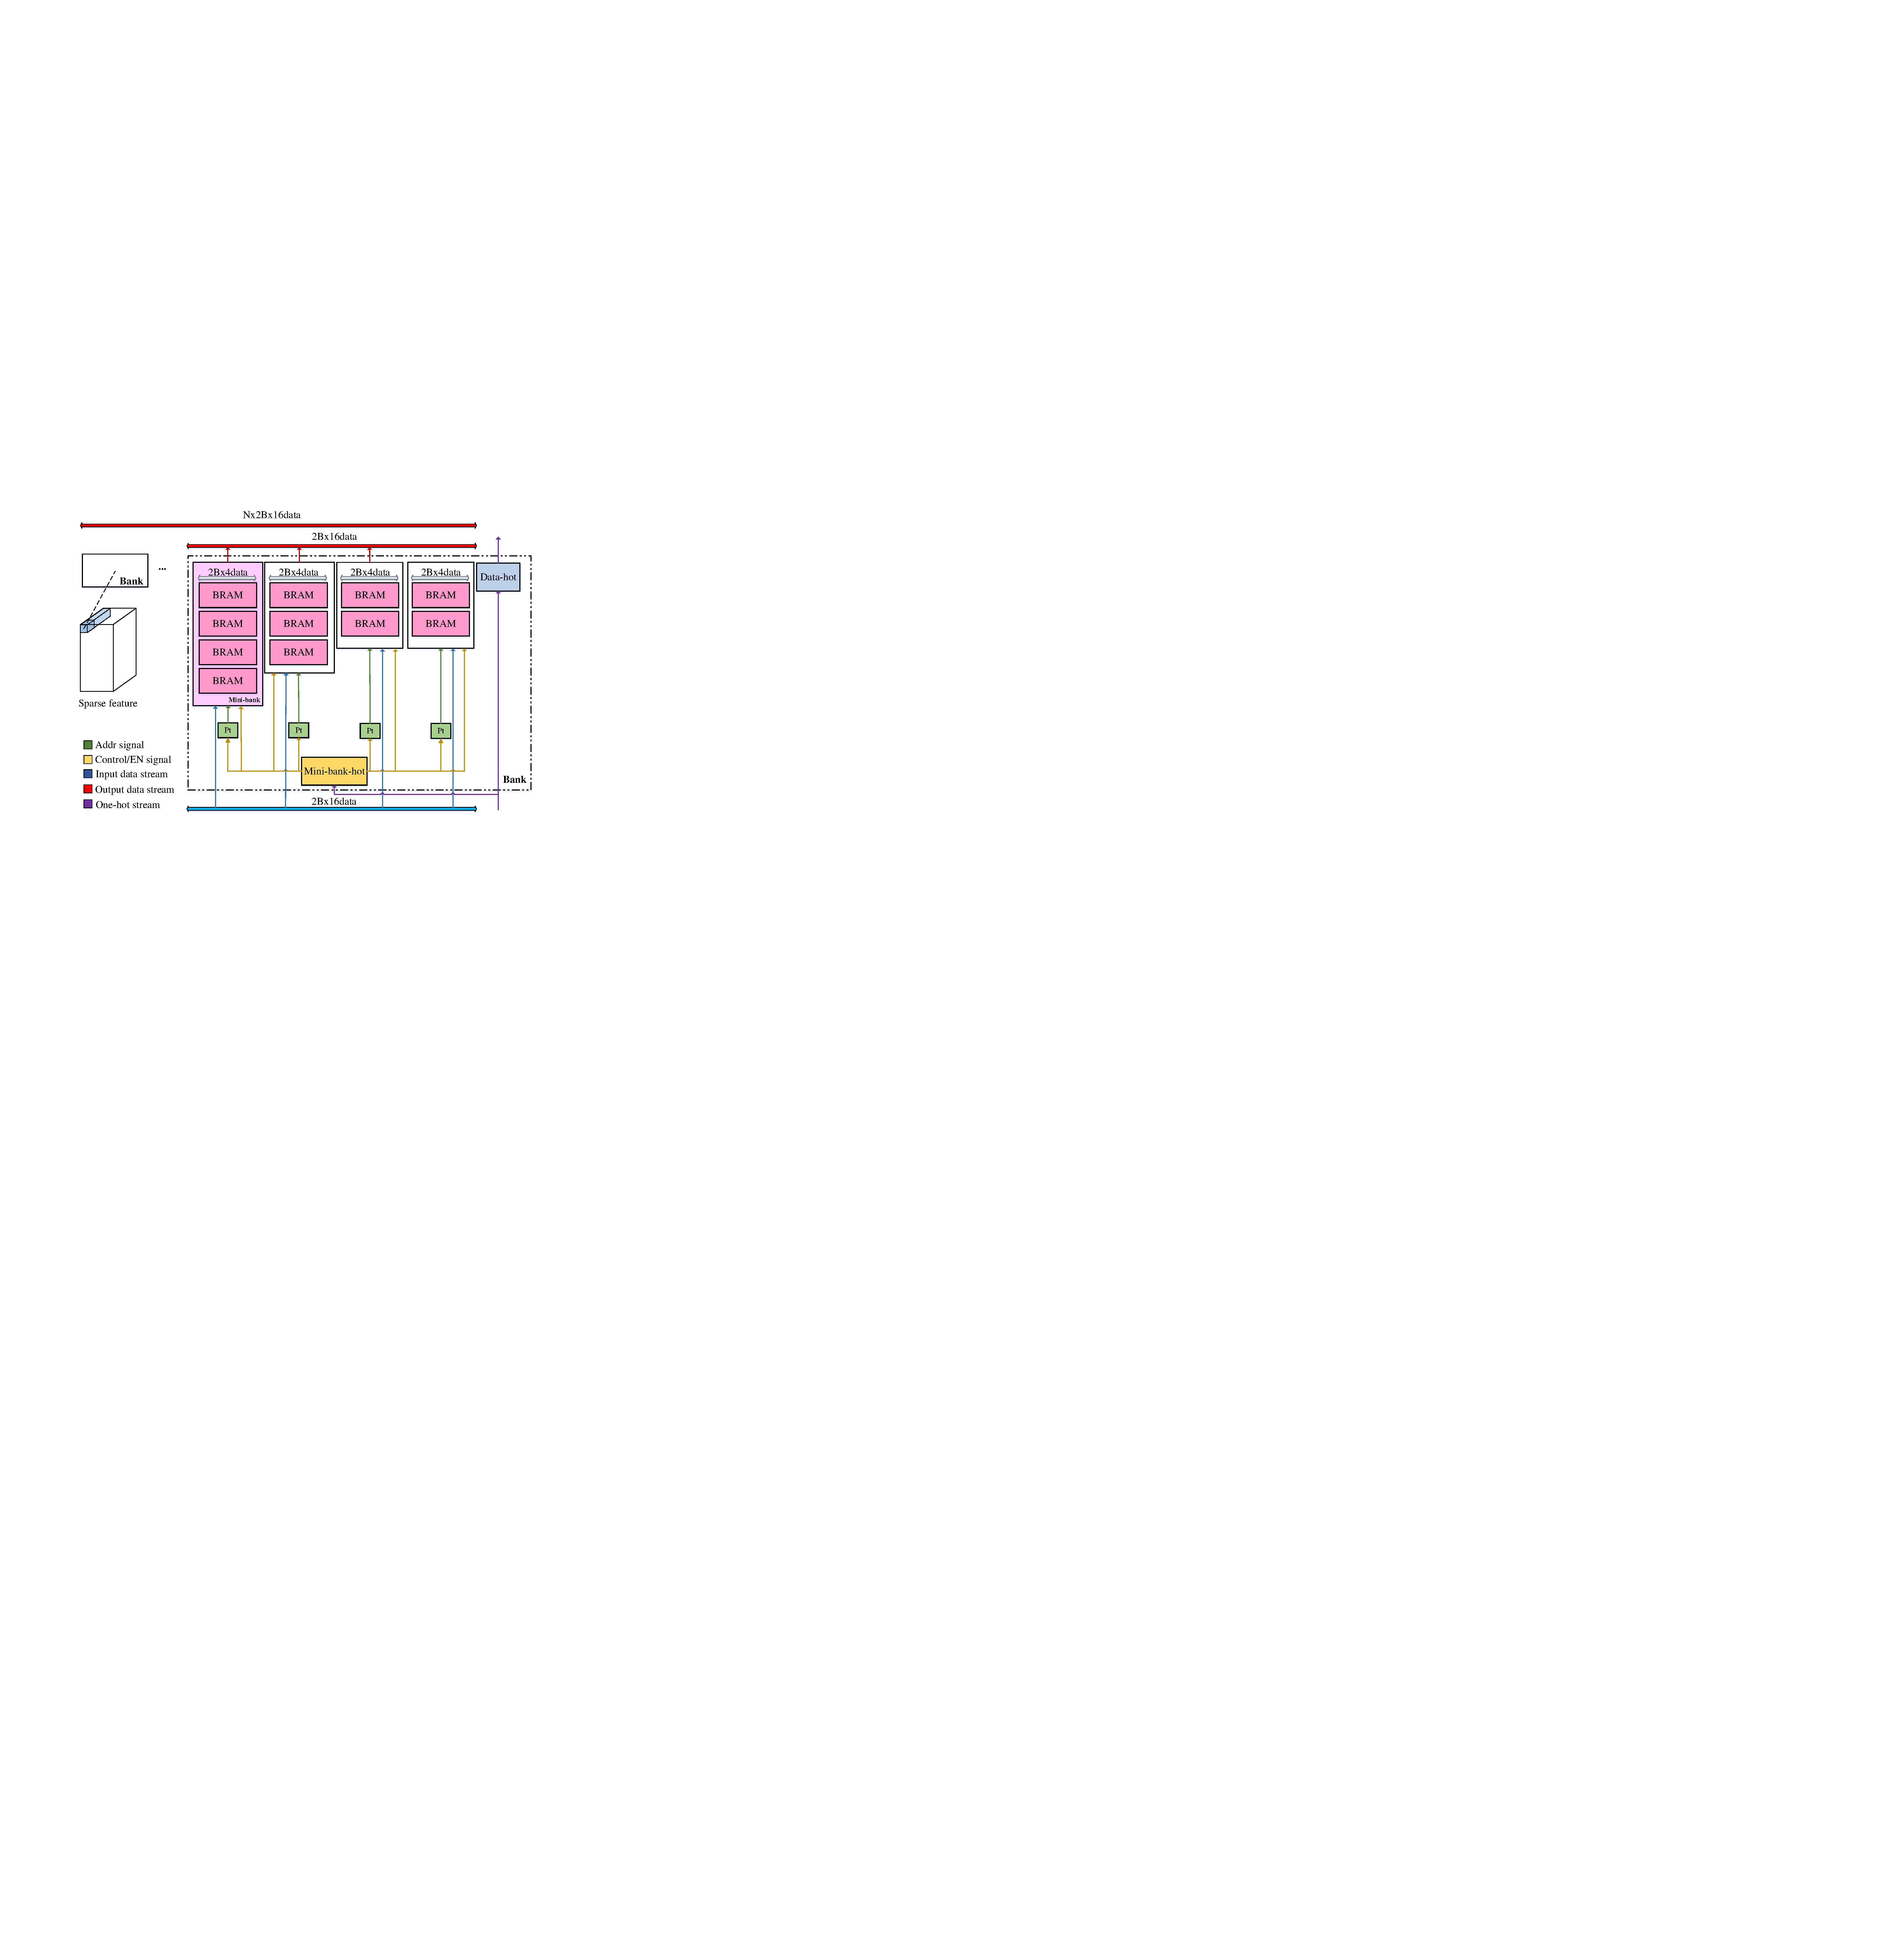
\includegraphics[width=0.42\textwidth]{myfig8.pdf}}
\caption{Illustration of TCM's dataflow.}\label{myfig8}
\end{figure}

\textbf{Storage:} The compact storage for sparse feature is consisted of bank storage units, which includes mini-banks, mini-bank-hot storage, data-hot storage and address controller: pt. The key insight of bank storage design is to keep access regularity on data-width dimension and reduce useless storage on data-depth direction. When input data and hot codes are valid, mbhot sends enabling signal to every mini-banks and related pt parts. For example, if the input data-hot code is 0001\_1100\_0000\_0111, thus there are five non-zero data in the high bits of input data stream and the mbhot is 1100. With zero-padding performed on lower bits, the first mini-bank receives and store four valid data, the second mini-bank keeps fifth valid data and three zero data. Their pt will self-add after this data-writing. Other mini-banks and their pt are not started and stay unchanged. Similarly, when we need to load data from bank storage in order, mbhot enables functional mini-banks and pts to output correct data. The disabled mini-banks�� output is covered by zero. By this way, compact data can be both stored and loaded in only one cycle without random access scheme.

Another issue on compact storage is to determine the volume of each mini-bank. Like deciding DSP's utilization, we can calculate the expectation of useful data based on offline sparsity. However, there always exists vectors with far more data density than average or far less data density than average. Denser vectors demand deeper mini-banks on the tail (the rightmost mini-bank in Fig.~\ref{myfig8}) while the lighter vectors merely occupy head mini-banks. In ideal cases, every vector is fit in bank-lines with no mini-banks unused and no vector truncated, but it is hard to precisely determine the number of valid data in every vector. Feature��s sparsity distribution of each layer can help us to adjust the depth of mini-banks. For example, sparsity of feature is 50\% and obey the normal distribution of. Guided by Three Sigma Code of normal distribution, it is estimated that 27\% of vectors has sparsity higher than 75\%, 23\%'s feature��s is between 50\%~75\%, 23\%'s data is between 25\%~50\% and 27\% vector's is below 25\%. The mini-bank arrangement in Fig.~\ref{myfig8} meets the demand of different density feature and reduces 31.25\% storage resource compared with sparse format. In actual design, BRAM units have variable grains, which provides higher storage efficiency and lower resource utilization.

\textbf{Decoding:} The decoding function is integrated in data-fetch module in SCM and TCM. Data-fetch not only controls loading address, but also translate compact data into sparse form. After receiving both data stream and data-hot codes from bank storages, parallel decoding modules perform on each banks�� output simultaneously. Each Translation part processes compressed feature in four pipeline stages, four data for one stage. Matched with encoding phase, the output of one bank is seen as the basic decoding grain, which further decreases the complexity of translation circuit. The sparse data finally is sent to feature-buffer and waits for computing.

\section{Experiments}
In this section, we evaluate our design on both software and hardware view. Our pruning method is explored on one NVIDIA V100 GPU using PyTorch, and accelerator architecture is implemented on Xilinx XCKU-115 with Vivado 2018.3 IDE.

\subsection{Validations on hybrid pruning method}
In our experiments, the proposed hybrid pruning method on 2s-AGCN model is compared with unstructured pruning and structured pruning. We also explore the impact of different pruning designs on accuracy, for example various fine-grained pruning schemes for temporal filters and channel-dropping modes in data reorganization phases.

\textit{Comparison:} Fig.~\ref{myfig9} illustrates the comparison results between our hybrid pruning methods and conventional unstructured pruning. With same parameters reduction rate, our method achieves better accuracy performance in most cases. Additionally, we apply 16bit quantization on our pruned models. With negligible accuracy loss, float data is transformed into 16bit fix-point format, where eight bits are allocated to decimal part and eight to integer part. To further accelerate the proposed application-specific system, half of input skeleton vectors is skipped. Although input-skip method lowers prediction accuracy, it brings 50\% reduction on total computation. Besides, the input-skip model with 86\% compress ratio still keeps the accuracy no less than original model, so we choose this model as final accelerating target.

\begin{figure}[htbp]
\centerline{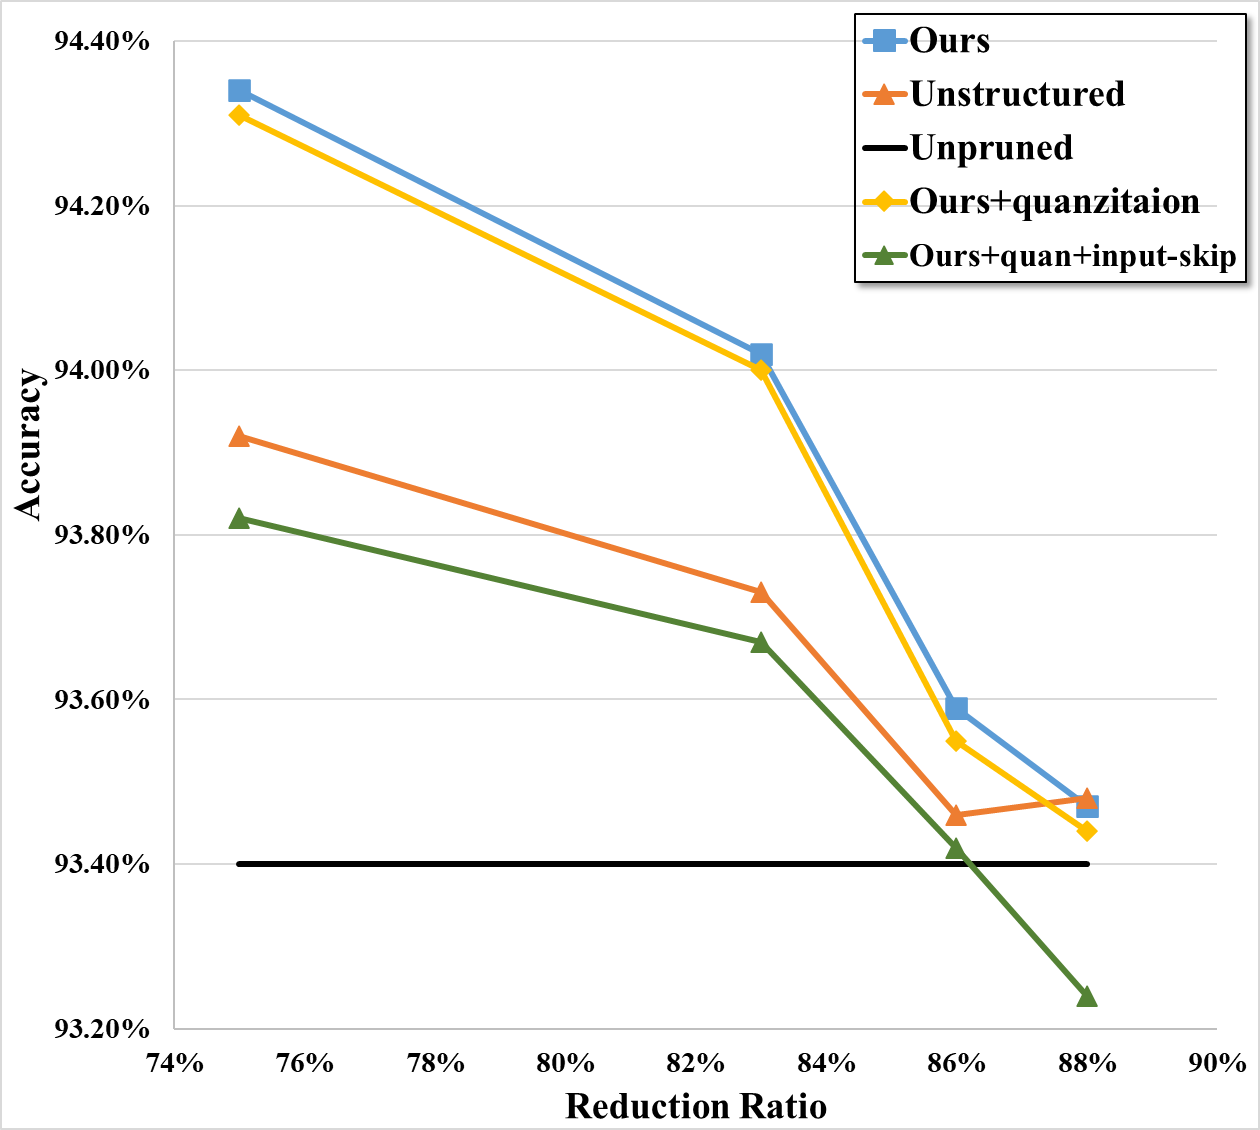
\includegraphics[width=6cm,height=3cm]{myfig9.png}}
\caption{Comparison results with unstructured pruning.}\label{myfig9}
\end{figure}

\textit{Exploration:} Both data reorganization and fine-grained temporal pruning are fatal to model accuracy, so to find the best pruning scheme, we conduct isolated experiments respectively. Guided by feature sparsity shown in Fig.~\ref{myfig1}, we set each layer��s channel dropping rate which roughly equals it��s sparsity respectively. For higher parameter reduction ratio, we progressively raise pruning rate on layers and observe effect on accuracy. Fig.~\ref{myfig10} demonstrates the channel-dropping results with details. The spatial convolutional parameter in block 1 is not pruned for it only has three input channels. Also, mix-grained pruning on temporal convolution is not performed to validate data reorganization method. It is revealed that with dropping rate shifting away from base sparsity, model reduction is growing while accuracy is decreasing. Considering mix-grained pruning needs data reorganization models as base, it is necessary to choose a conservative dropping scheme with higher.

\begin{figure}[htbp]
\centerline{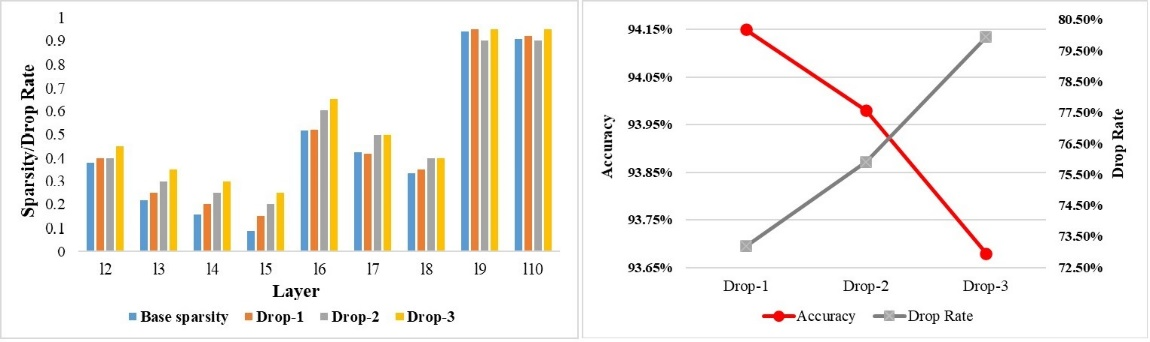
\includegraphics[width=8.5cm,height=3.5cm]{myfig10.png}}
\caption{Exploration on channel dropping.}\label{myfig10}
\end{figure}
The fine-grained pruning is important in holding accuracy and keeping balanced-weight, since coarse-grained pruning is totally decided by data reorganization. We carry out several experiments on fine-grained pruning details, including different pruning intervals, offsets and pruning rates. All experiments are based on Drop-1 model in fig. 9 and results are shown in Fig.~\ref{myfig11}. Pruning schemes in Fig.~\ref{myfig11} are named as the combination of cav (cavity), pruning rate (50, 67 for instance) and intra-order. Cav-70-1 means the first cavity patterns with 70\% reduction rate. With reduction rates goes higher, model bears more accuracy loss in general. However, cavity patterns play an important role as well. Having compress ratio of 70\%, cav-70-1 performs better than cav-70-2 on performance for more balanced weight pruning. Every weight line in cav-70-1 has two or three sampling chances, while in cav-70-2, different lines can be kept from one time to four times. Balanced pruning schemes not only provide convenience for hardware, but also ensure the accuracy performance. The same situation happens between cav-75-1 and cav-75-2 too. Taking both compress ratio and accuracy into consideration, cav-70-1 is chosen to be the final design.

\begin{figure}[htbp]
\centerline{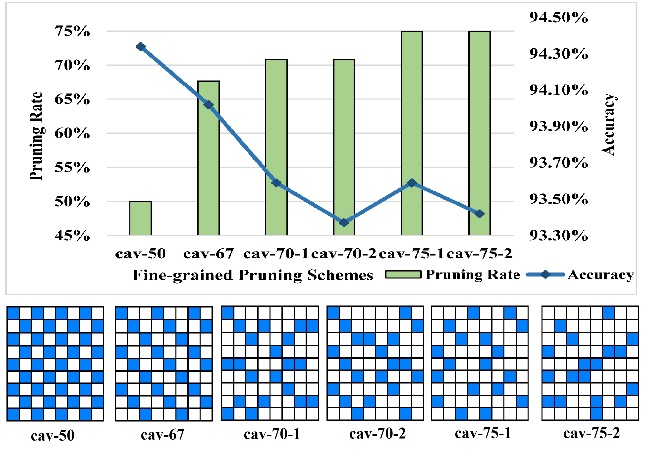
\includegraphics[width=0.45\textwidth]{myfig11.png}}
\caption{Exploration on fine-grained pruning schemes.}\label{myfig11}
\end{figure}

\subsection{Hardware implement}
\textit{Dyn-MultPE:} Dyn-MultPE works on the cav-70-1 cavity pattern, which means there are three Dyn-MultPEs processing six waiting queues and six processing four waiting queues. Based on eq. 5, different numbers of DSPs are settled in each layer��s Dyn-MultPEs. We also adjust the number of temporal convolutional PE to keep balance between pipeline stages. The detailed information is illustrated in Table.~\ref{tab2}, where our dynamic data scheduling trades only 6.48\% longer delay for DSP reduction of 23.24\%.

\begin{table}[htbp]
\caption{Utilization, working efficiency and max delay of Dyn-MultPE.}
\begin{center}
\begin{tabular}{|c|c|c|c|c|}
\hline
layer&DSP in one PE\%&total DSP&efficiency &max delay\\
\hline
1&4/6&63&66.79\%&0\\
\hline
2&4/6&126&83.76\%&3.70\%\\
\hline
3&4/6&126&80.96\%&0\\
\hline
4&2/3&126&83.46\%&7.40\%\\
\hline
5&2/3&126&70.35\%&0\\
\hline
6&2/3&63&78.73\%&0.50\%\\
\hline
7&1/2&63&86.81\%&7.40\%\\
\hline
8&1/2&63&49.54\%&0\\
\hline
9&1/2&63&85.50\%&14.00\%\\
\hline
10&1/2&63&67.85\%&0\\
\hline
total&&882&75.38\%&6.48\%\\
\hline
static&&1149&57.86\%&0\\
\hline
\end{tabular}
\label{tab2}
\end{center}
\end{table}

\textit{RFC:} as stated above, RFC design relies on sparsity distribution. To optimize runtime compress storage, we refer to offline statistic information, which is shown in Table.~\ref{tab3}. Feature vectors are divided into four categories by their sparsity: 75\%~100\% (I), 50\%~75\% (II), 25\%~50\% (III) and 0\%~25\% (IV). According to our RFC design, vector of first category occupies one mini-bank, ones in II takes two, III takes three and IV takes four mini-banks. We can thus get the total BRAM blocks used for RFC structure. Comparison in fig. 11 indicates that our RFC design brings 35.93\% reduction on occupied BRAM blocks. Moreover, with almost equal amount of used BRAM elements, RFC can finish data-loading in one cycle and encoding/decoding in four cycles, while CSC format usually needs 64 cycles to load data or decoding data in serial. With less extra hardware cost and similar storage compress ratio, RFC structure achieves more regular data-access.


\begin{table}[htbp]
\caption{.}
\begin{center}
\begin{tabular}{|c|c|c|c|c|}
\hline
layer&I&II&III&IV\\
\hline
l1.sconv&$<$0.01\%&29.35\%&70.64\%&$<$0.01\%\\
\hline
l1.tconv&0.02\%&94.73\%&5.25\%&0.00\%\\
\hline
l2.sconv&0.00\%&0.73\%&75.79\%&23.48\%\\
\hline
l2.tconv&$<$0.01\%&34.24\%&65.76\%&0.00\%\\
\hline
l3.sconv&0.00\%&1.24\%&90.00\%&8.75\%\\
\hline
l3.tconv&0.00\%&3.54\%&96.45\%&$<$0.01\%\\
\hline
l4.sconv&0.00\%&0.62\%&89.75\%&9.62\%\\
\hline
l4.tconv&0.00\%&0.16\%&57.60\%&42.24\%\\
\hline
l5.sconv&0.47\%&79.01\%&20.52\%&$<$0.01\%\\
\hline
l5.tconv&0.05\%&99.91\%&0.05\%&0.00\%\\
\hline
l6.sconv&$<$0.01\%&62.97\%&37.03\%&$<$0.01\%\\
\hline
l6.tconv&$<$0.01\%&68.91\%&31.09\%&0.00\%\\
l7.sconv&0.01\%&40.06\%&59.74\%&0.19\%\\
\hline
l7.tconv&0.00\%&8.31\%&83.96\%&7.74\%\\
\hline
l8.sconv&87.05\%&12.95\%&0.00\%&0.00\%\\
\hline
l8.tconv&100.00\%&0.00\%&0.00\%&0.00\%\\
\hline
l9.sconv&0.73\%&99.20\%&0.07\%&0.00\%\\
\hline
l9.tconv&100.00\%&0.00\%&0.00\%&0.00\%\\
l10.sconv&29.49\%&70.51\%&0.00\%&0.00\%\\
\hline
\end{tabular}
\label{tab3}
\end{center}
\end{table}

\begin{figure}[htbp]
\centerline{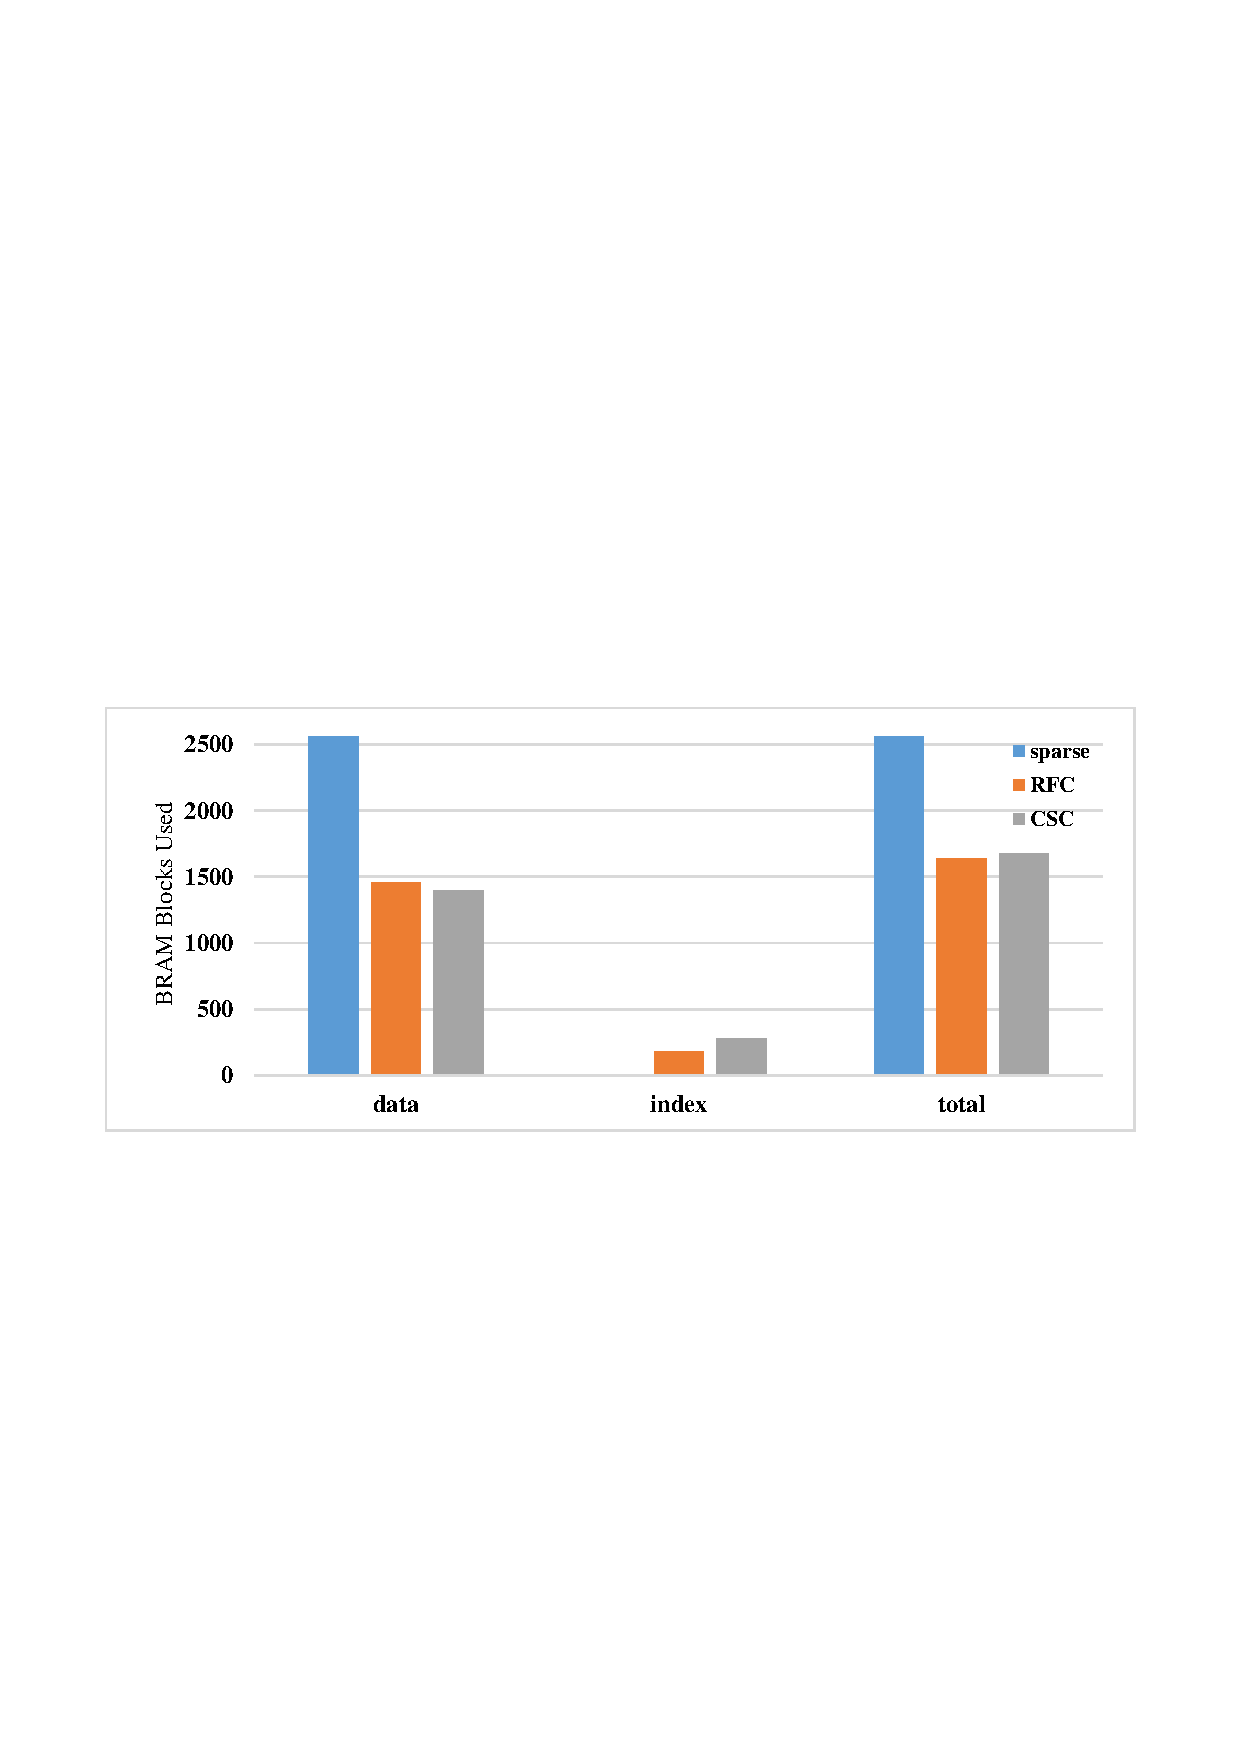
\includegraphics[width=0.45\textwidth]{myfig12.pdf}}
\caption{Storage cost of three data formats.}\label{myfig12}
\end{figure}
Overall performance: Our architecture is implemented on Xilinx XCKU-115 with frequency of 172MHz. The resource utilization is demonstrated in Table.~ref{tab4}, together with comparison with FDU. Despite more hardware resource is utilized by our RFC-HyGCN, experiments have proved that our design has superiority on peak performance, throughput and DSP efficiency. In table. 6, we compare the peak performance of ours and two high-end GPUs. The ��original�� in the table means testing program is the original version of 2s-AGCN, the ��wo-C�� means the optimized version without C\_k matrix, and the ��skip�� means input-skipping is applied on model. To fully use the memory in GPUs, target model runs with 200 or 700 samples in one batch on 2080Ti and V100, respectively. Compared with two main-stream GPUs, our accelerator provides 1.36x~9.47x of speedup, showing competitive performance.

\begin{table*}[htbp]
\caption{Comparison between ours and FDU.}
\begin{center}
\begin{tabular}{|c|c|c|c|c|c|c|c|}
\hline
&dsp&bram blocks&LUT&dsp efficiency &peak perf &frequency & fps\\
\hline
ours&3544&1806&176776&0.322GOP/s/DSP &1142GOP/S&172Mhz&271.25\\
\hline
fdu&228&151&44457&0.202GOP/s/DSP &46GOP/S&188Mhz&11.99\\
\hline
\end{tabular}
\label{tab4}
\end{center}
\end{table*}

\begin{table*}[htbp]
\caption{Performance comparison between ours and high-end GPUs.}
\begin{center}
\begin{tabular}{|c|c|c|c|c|c|c|c|}
\hline
&ours&2080Ti-original&V100-original&2080Ti-woC&V100-woC&2080Ti-skip&V100-skip\\
\hline
throughput&271.25&28.63&45.08&69.38&98.87&141&199.09\\
\hline
speed-up&&9.47&6.02&3.91&2.74&1.92&1.36\\
\hline
\end{tabular}
\label{tab5}
\end{center}
\end{table*}

\section{Conclusion}
In this article, we propose a software-hardware co-design work: RFC-HyGCN, including hybrid pruning method and a runtime sparse feature compress architecture with layer-pipeline. We explore a hybrid pruning method specific on action recognition GCNs to purse skipping both graph and convolution computation. Moreover, we propose an architecture based on balanced pruned model. In addition, we design runtime sparse feature compact format to reduce zero-storage between layers. Experiments demonstrate that compared with conventional structured unstructured pruning, our method achieves better accuracy performance in most cases. The accelerator is implemented on Xilinx XCKU-115 FPGA, at the cost of negligible encoding/decoding cost, RFC reduces 35.93\% of BRAM blocks and 23.24\% of DSPs. Compared with another work on accelerating action recognition GCNs, ours provides 22.62x speed-up and 59.41\% elevation on DSP efficiency. On contrast to high-end GPUs, RFC-HyGCN achieves 1.36x~9.47x speed-up on throughput.
%
%The IEEEtran class file is used to format your paper and style the text. All margins,
%column widths, line spaces, and text fonts are prescribed; please do not
%alter them. You may note peculiarities. For example, the head margin
%measures proportionately more than is customary. This measurement
%and others are deliberate, using specifications that anticipate your paper
%as one part of the entire proceedings, and not as an independent document.
%Please do not revise any of the current designations.
%
%\section{Prepare Your Paper Before Styling}
%Before you begin to format your paper, first write and save the content as a
%separate text file. Complete all content and organizational editing before
%formatting. Please note sections \ref{AA}--\ref{SCM} below for more information on
%proofreading, spelling and grammar.
%
%Keep your text and graphic files separate until after the text has been
%formatted and styled. Do not number text heads---{\LaTeX} will do that
%for you.
%
%\subsection{Abbreviations and Acronyms}\label{AA}
%Define abbreviations and acronyms the first time they are used in the text,
%even after they have been defined in the abstract. Abbreviations such as
%IEEE, SI, MKS, CGS, ac, dc, and rms do not have to be defined. Do not use
%abbreviations in the title or heads unless they are unavoidable.
%
%\subsection{Units}
%\begin{itemize}
%\item Use either SI (MKS) or CGS as primary units. (SI units are encouraged.) English units may be used as secondary units (in parentheses). An exception would be the use of English units as identifiers in trade, such as ``3.5-inch disk drive''.
%\item Avoid combining SI and CGS units, such as current in amperes and magnetic field in oersteds. This often leads to confusion because equations do not balance dimensionally. If you must use mixed units, clearly state the units for each quantity that you use in an equation.
%\item Do not mix complete spellings and abbreviations of units: ``Wb/m\textsuperscript{2}'' or ``webers per square meter'', not ``webers/m\textsuperscript{2}''. Spell out units when they appear in text: ``. . . a few henries'', not ``. . . a few H''.
%\item Use a zero before decimal points: ``0.25'', not ``.25''. Use ``cm\textsuperscript{3}'', not ``cc''.)
%\end{itemize}
%
%\subsection{Equations}
%Number equations consecutively. To make your
%equations more compact, you may use the solidus (~/~), the exp function, or
%appropriate exponents. Italicize Roman symbols for quantities and variables,
%but not Greek symbols. Use a long dash rather than a hyphen for a minus
%sign. Punctuate equations with commas or periods when they are part of a
%sentence, as in:
%\begin{equation}
%a+b=\gamma\label{eq}
%\end{equation}
%
%Be sure that the
%symbols in your equation have been defined before or immediately following
%the equation. Use ``\eqref{eq}'', not ``Eq.~\eqref{eq}'' or ``equation \eqref{eq}'', except at
%the beginning of a sentence: ``Equation \eqref{eq} is . . .''
%
%\subsection{\LaTeX-Specific Advice}
%
%Please use ``soft'' (e.g., \verb|\eqref{Eq}|) cross references instead
%of ``hard'' references (e.g., \verb|(1)|). That will make it possible
%to combine sections, add equations, or change the order of figures or
%citations without having to go through the file line by line.
%
%Please don't use the \verb|{eqnarray}| equation environment. Use
%\verb|{align}| or \verb|{IEEEeqnarray}| instead. The \verb|{eqnarray}|
%environment leaves unsightly spaces around relation symbols.
%
%Please note that the \verb|{subequations}| environment in {\LaTeX}
%will increment the main equation counter even when there are no
%equation numbers displayed. If you forget that, you might write an
%article in which the equation numbers skip from (17) to (20), causing
%the copy editors to wonder if you've discovered a new method of
%counting.
%
%{\BibTeX} does not work by magic. It doesn't get the bibliographic
%data from thin air but from .bib files. If you use {\BibTeX} to produce a
%bibliography you must send the .bib files.
%
%{\LaTeX} can't read your mind. If you assign the same label to a
%subsubsection and a table, you might find that Table I has been cross
%referenced as Table IV-B3.
%
%{\LaTeX} does not have precognitive abilities. If you put a
%\verb|\label| command before the command that updates the counter it's
%supposed to be using, the label will pick up the last counter to be
%cross referenced instead. In particular, a \verb|\label| command
%should not go before the caption of a figure or a table.
%
%Do not use \verb|\nonumber| inside the \verb|{array}| environment. It
%will not stop equation numbers inside \verb|{array}| (there won't be
%any anyway) and it might stop a wanted equation number in the
%surrounding equation.
%
%\subsection{Some Common Mistakes}\label{SCM}
%\begin{itemize}
%\item The word ``data'' is plural, not singular.
%\item The subscript for the permeability of vacuum $\mu_{0}$, and other common scientific constants, is zero with subscript formatting, not a lowercase letter ``o''.
%\item In American English, commas, semicolons, periods, question and exclamation marks are located within quotation marks only when a complete thought or name is cited, such as a title or full quotation. When quotation marks are used, instead of a bold or italic typeface, to highlight a word or phrase, punctuation should appear outside of the quotation marks. A parenthetical phrase or statement at the end of a sentence is punctuated outside of the closing parenthesis (like this). (A parenthetical sentence is punctuated within the parentheses.)
%\item A graph within a graph is an ``inset'', not an ``insert''. The word alternatively is preferred to the word ``alternately'' (unless you really mean something that alternates).
%\item Do not use the word ``essentially'' to mean ``approximately'' or ``effectively''.
%\item In your paper title, if the words ``that uses'' can accurately replace the word ``using'', capitalize the ``u''; if not, keep using lower-cased.
%\item Be aware of the different meanings of the homophones ``affect'' and ``effect'', ``complement'' and ``compliment'', ``discreet'' and ``discrete'', ``principal'' and ``principle''.
%\item Do not confuse ``imply'' and ``infer''.
%\item The prefix ``non'' is not a word; it should be joined to the word it modifies, usually without a hyphen.
%\item There is no period after the ``et'' in the Latin abbreviation ``et al.''.
%\item The abbreviation ``i.e.'' means ``that is'', and the abbreviation ``e.g.'' means ``for example''.
%\end{itemize}
%An excellent style manual for science writers is \cite{b7}.
%
%\subsection{Authors and Affiliations}
%\textbf{The class file is designed for, but not limited to, six authors.} A
%minimum of one author is required for all conference articles. Author names
%should be listed starting from left to right and then moving down to the
%next line. This is the author sequence that will be used in future citations
%and by indexing services. Names should not be listed in columns nor group by
%affiliation. Please keep your affiliations as succinct as possible (for
%example, do not differentiate among departments of the same organization).
%
%\subsection{Identify the Headings}
%Headings, or heads, are organizational devices that guide the reader through
%your paper. There are two types: component heads and text heads.
%
%Component heads identify the different components of your paper and are not
%topically subordinate to each other. Examples include Acknowledgments and
%References and, for these, the correct style to use is ``Heading 5''. Use
%``figure caption'' for your Figure captions, and ``table head'' for your
%table title. Run-in heads, such as ``Abstract'', will require you to apply a
%style (in this case, italic) in addition to the style provided by the drop
%down menu to differentiate the head from the text.
%
%Text heads organize the topics on a relational, hierarchical basis. For
%example, the paper title is the primary text head because all subsequent
%material relates and elaborates on this one topic. If there are two or more
%sub-topics, the next level head (uppercase Roman numerals) should be used
%and, conversely, if there are not at least two sub-topics, then no subheads
%should be introduced.
%
%\subsection{Figures and Tables}
%\paragraph{Positioning Figures and Tables} Place figures and tables at the top and
%bottom of columns. Avoid placing them in the middle of columns. Large
%figures and tables may span across both columns. Figure captions should be
%below the figures; table heads should appear above the tables. Insert
%figures and tables after they are cited in the text. Use the abbreviation
%``Fig.~\ref{fig}'', even at the beginning of a sentence.
%
%\begin{table}[htbp]
%\caption{Table Type Styles}
%\begin{center}
%\begin{tabular}{|c|c|c|c|}
%\hline
%\textbf{Table}&\multicolumn{3}{|c|}{\textbf{Table Column Head}} \\
%\cline{2-4}
%\textbf{Head} & \textbf{\textit{Table column subhead}}& \textbf{\textit{Subhead}}& \textbf{\textit{Subhead}} \\
%\hline
%copy& More table copy$^{\mathrm{a}}$& &  \\
%\hline
%\multicolumn{4}{l}{$^{\mathrm{a}}$Sample of a Table footnote.}
%\end{tabular}
%\label{tab1}
%\end{center}
%\end{table}
%
%\begin{figure}[htbp]
%\centerline{
\includegraphics{fig1.png}}
%\caption{Example of a figure caption.}
%\label{fig}
%\end{figure}
%
%Figure Labels: Use 8 point Times New Roman for Figure labels. Use words
%rather than symbols or abbreviations when writing Figure axis labels to
%avoid confusing the reader. As an example, write the quantity
%``Magnetization'', or ``Magnetization, M'', not just ``M''. If including
%units in the label, present them within parentheses. Do not label axes only
%with units. In the example, write ``Magnetization (A/m)'' or ``Magnetization
%\{A[m(1)]\}'', not just ``A/m''. Do not label axes with a ratio of
%quantities and units. For example, write ``Temperature (K)'', not
%``Temperature/K''.

\section*{Acknowledgment}

The preferred spelling of the word ``acknowledgment'' in America is without
an ``e'' after the ``g''. Avoid the stilted expression ``one of us (R. B.
G.) thanks $\ldots$''. Instead, try ``R. B. G. thanks$\ldots$''. Put sponsor
acknowledgments in the unnumbered footnote on the first page.

%\section*{References}
%
%Please number citations consecutively within brackets \cite{b1}. The
%sentence punctuation follows the bracket \cite{b2}. Refer simply to the reference
%number, as in \cite{b3}---do not use ``Ref. \cite{b3}'' or ``reference \cite{b3}'' except at
%the beginning of a sentence: ``Reference \cite{b3} was the first $\ldots$''
%
%Number footnotes separately in superscripts. Place the actual footnote at
%the bottom of the column in which it was cited. Do not put footnotes in the
%abstract or reference list. Use letters for table footnotes.
%
%Unless there are six authors or more give all authors' names; do not use
%``et al.''. Papers that have not been published, even if they have been
%submitted for publication, should be cited as ``unpublished'' \cite{b4}. Papers
%that have been accepted for publication should be cited as ``in press'' \cite{b5}.
%Capitalize only the first word in a paper title, except for proper nouns and
%element symbols.
%
%For papers published in translation journals, please give the English
%citation first, followed by the original foreign-language citation \cite{b6}.

%\begin{thebibliography}{00}
%\bibitem{b1} G. Eason, B. Noble, and I. N. Sneddon, ``On certain integrals of Lipschitz-Hankel type involving products of Bessel functions,'' Phil. Trans. Roy. Soc. London, vol. A247, pp. 529--551, April 1955.
%\bibitem{b2} J. Clerk Maxwell, A Treatise on Electricity and Magnetism, 3rd ed., vol. 2. Oxford: Clarendon, 1892, pp.68--73.
%\bibitem{b3} I. S. Jacobs and C. P. Bean, ``Fine particles, thin films and exchange anisotropy,'' in Magnetism, vol. III, G. T. Rado and H. Suhl, Eds. New York: Academic, 1963, pp. 271--350.
%\bibitem{b4} K. Elissa, ``Title of paper if known,'' unpublished.
%\bibitem{b5} R. Nicole, ``Title of paper with only first word capitalized,'' J. Name Stand. Abbrev., in press.
%\bibitem{b6} Y. Yorozu, M. Hirano, K. Oka, and Y. Tagawa, ``Electron spectroscopy studies on magneto-optical media and plastic substrate interface,'' IEEE Transl. J. Magn. Japan, vol. 2, pp. 740--741, August 1987 [Digests 9th Annual Conf. Magnetics Japan, p. 301, 1982].
%\bibitem{b7} M. Young, The Technical Writer's Handbook. Mill Valley, CA: University Science, 1989.
%\end{thebibliography}
\bibliographystyle{ieeetr}
\bibliography{inerbib}
\vspace{12pt}
\color{red}
IEEE conference templates contain guidance text for composing and formatting conference papers. Please ensure that all template text is removed from your conference paper prior to submission to the conference. Failure to remove the template text from your paper may result in your paper not being published.

\end{document}
